% Module 1: What This Is and What You Can Do With It
% Beamer Presentation — Claude Code for Academic Researchers
\documentclass[aspectratio=169, 11pt]{beamer}

% ── Theme and Colors ──────────────────────────────────────────────
\usetheme{Madrid}
\usecolortheme{default}

% Custom colors
\definecolor{anthropic}{RGB}{50, 50, 80}
\definecolor{accent}{RGB}{180, 90, 40}
\definecolor{lightgray}{RGB}{245, 245, 245}

\setbeamercolor{structure}{fg=anthropic}
\setbeamercolor{frametitle}{bg=anthropic, fg=white}
\setbeamercolor{title}{bg=anthropic, fg=white}
\setbeamercolor{block title}{bg=anthropic, fg=white}
\setbeamercolor{block body}{bg=lightgray}
\setbeamercolor{alerted text}{fg=accent}

\setbeamerfont{title}{size=\Large, series=\bfseries}
\setbeamerfont{frametitle}{size=\large, series=\bfseries}

% ── Packages ──────────────────────────────────────────────────────
\usepackage{graphicx}
\usepackage{booktabs}
\usepackage{listings}
\usepackage{fontenc}
\usepackage{hyperref}
\usepackage{tikz}

\lstset{
  basicstyle=\ttfamily\small,
  backgroundcolor=\color{lightgray},
  frame=single,
  framerule=0pt,
  breaklines=true,
  columns=fullflexible,
  literate={_}{\_}1,
}

% ── Metadata ──────────────────────────────────────────────────────
\title{Claude Code for Academic Researchers}
\subtitle{A Methods Workshop in AI-Assisted Research}
\author{Brady Allardice}
\date{}
\institute{UPF \& IBEI}

% ══════════════════════════════════════════════════════════════════
\begin{document}

% ── Course Title ──────────────────────────────────────────────────
\begin{frame}[plain]
  \titlepage
\end{frame}

% ── About the Instructor ─────────────────────────────────────────
\begin{frame}{About Me}
  \begin{columns}[T]
    \begin{column}{0.52\textwidth}
      \textbf{Brady Allardice}\\
      PhD Candidate, Political \& Social Sciences\\
      UPF / IBEI, Barcelona

      \vspace{0.5em}
      \textbf{Research:} Political economy of technological change
      \begin{itemize}
        \item Automation, AI, and political behavior
        \item LLM-based text classification pipelines
      \end{itemize}

      \vspace{0.5em}
      \textbf{Background:}
      \begin{itemize}
        \item M.Res.\ Political Science (UPF)
        \item M.Sc.\ Economics (Barcelona School of Economics)
        \item Former data scientist
      \end{itemize}
    \end{column}
    \begin{column}{0.44\textwidth}
      \textbf{Why this course:}
      \begin{itemize}
        \item Daily user of Claude Code for academic research
        \item Use it across the full pipeline: data cleaning, analysis, robustness checks, code auditing, replication, writing, reviewing
        \item These tools can dramatically expand what a researcher can accomplish, if used with the right workflows
      \end{itemize}

      \vspace{0.5em}
      {\small brady.allardice@upf.edu\\github.com/bradyall}
    \end{column}
  \end{columns}
\end{frame}

% ── Participant Introductions ────────────────────────────────────
\begin{frame}{Introductions}
  \begin{enumerate}
    \item Who are you? {\small (name, department, research area)}
    \item What does your daily workflow look like? {\small (tools, languages, data)}
    \item How do you currently use AI, if at all?
    \item What do you hope to learn from this course?
  \end{enumerate}
\end{frame}

% ── Course Overview ───────────────────────────────────────────────
\begin{frame}{Course Roadmap}
  \small
  \begin{tabular}{@{}c p{0.82\textwidth}@{}}
    \toprule
    \textbf{Session} & \textbf{Focus} \\
    \midrule
    1 & Introduction: what Claude Code is, what you can do with it, and how it works \\
    \midrule
    2 & Research pipelines: from data to results --- cleaning, estimation, robustness, \LaTeX{} tables \\
    \midrule
    3 & Git and \LaTeX{} in VS Code: version control and the integrated research environment \\
    \midrule
    4 & Advanced Claude Code: skills and MCPs (Zotero, GitHub) \\
    \midrule
    5 & Subagents, hooks, and the final project \\
    \bottomrule
  \end{tabular}

  \vspace{0.6em}
  {\footnotesize 5 sessions $\times$ 2 hours \quad$\vert$\quad 60--70\% hands-on \quad$\vert$\quad Pair programming throughout}
\end{frame}

\begin{frame}{Core Framework}
  \begin{alertblock}{The Central Idea}
    You are the principal investigator. Claude Code is the research assistant.\\
    You direct the work, make analytical decisions, and verify every result.\\
    Claude Code handles the mechanical execution.
  \end{alertblock}

  \vspace{0.5em}
  The question is never ``can Claude Code do this.'' It almost always can.

  \vspace{0.3em}
  The question is: \textbf{what is the most productive and reliable way to get this done?}

  \vspace{0.8em}
  \textbf{By the end of this course, you will be able to:}
  \begin{itemize}
    \item Automate data cleaning, robustness checks, code auditing, and documentation
    \item Choose the right execution mode for each task
    \item Verify output against known properties of your data
    \item Recognize when Claude Code is failing and intervene effectively
  \end{itemize}
\end{frame}

% ══════════════════════════════════════════════════════════════════
%  MODULE 1 BEGINS
% ══════════════════════════════════════════════════════════════════

\begin{frame}[plain]
  \centering
  \vfill
  {\Large\textbf{Module 1}}\\[0.5em]
  {\large What This Is and What You Can Do With It}\\[0.3em]
  {\small Demo + Exercise}
  \vfill
\end{frame}

% ══════════════════════════════════════════════════════════════════
%  GET THE CODE
% ══════════════════════════════════════════════════════════════════

\begin{frame}[fragile]{How We'll Work: Your Own Workspace}
  The course materials live in one shared repo, organized as self-contained session folders:

  \vspace{0.3em}
  \begin{lstlisting}[basicstyle=\ttfamily\footnotesize]
claude-code-workshop/
  session_1/     <- today's materials live here
  session_2/
  session_3/
  ...
  \end{lstlisting}

  \vspace{0.4em}
  \textbf{The workflow, every session:} copy that session's folder out of the repo into your own workspace, and work there. The shared repo stays read-only for you.

  \vspace{0.4em}
  \begin{block}{Why}
    I can push new material anytime without breaking your work. You can edit, break, delete, and redo without worrying about the shared state. No merge conflicts.
  \end{block}
\end{frame}

\begin{frame}[fragile]{The Start-of-Session Ritual}
  \textbf{Do this at the start of every session.} Today is the first time:

  \vspace{0.4em}
  \begin{lstlisting}[basicstyle=\ttfamily\footnotesize]
# 1. Get the course repo (first time: clone it)
git clone https://github.com/bradyallardice/claude-code-workshop.git
cd claude-code-workshop

# 2. Make your workspace and copy today's folder into it
mkdir -p ~/my_workspace
cp -r session_1/ ~/my_workspace/session_1/

# 3. Open your copy in VS Code and work there
cd ~/my_workspace/session_1 && code .
  \end{lstlisting}

  \vspace{0.3em}
  {\small \textbf{Already have the repo from pre-work?} Run \texttt{git pull} inside it instead of cloning, then continue with Steps 2--3.}

  \vspace{0.3em}
  \textbf{We do it together now, live.} Everyone ends up in the same clean state before we move on.
\end{frame}

% ══════════════════════════════════════════════════════════════════
%  SETUP CHECK
% ══════════════════════════════════════════════════════════════════

\begin{frame}{Setup Check}
  Open the terminal in VS Code (or your standalone terminal) and run:

  \vspace{0.5em}
  \begin{enumerate}
    \item Verify Node.js: \lstinline{node --version}
    \item Verify Claude Code: \lstinline{claude --version}
    \item Launch Claude Code: \lstinline{claude}
  \end{enumerate}

  \vspace{0.8em}
  You should see Claude Code's interface appear in your terminal.

  \vspace{0.5em}
  Try typing a simple message: \lstinline{What files are in this directory?}

  \vspace{1em}
  \textbf{If you completed pre-work:} help your neighbor.\\
  \textbf{If you're stuck:} pair with someone who is set up. We'll troubleshoot at break.
\end{frame}

% ══════════════════════════════════════════════════════════════════
%  OPENING DEMO  [0:00–2:00]
% ══════════════════════════════════════════════════════════════════

\begin{frame}{Live Demo: The Data}
  \textbf{Dataset 1: County Presidential Election Returns}
  \begin{itemize}
    \item Source: MIT Election Data + Science Lab
    \item County-level vote totals by candidate and party, 2000--2024
    \item ${\sim}$94{,}000 rows, one row per county $\times$ year $\times$ candidate
    \item Variables: FIPS codes, candidate names, party, vote counts, vote mode
  \end{itemize}

  \vspace{0.5em}
  \textbf{Dataset 2: IPUMS American Community Survey Microdata}
  \begin{itemize}
    \item Source: IPUMS USA (University of Minnesota)
    \item Person-level survey records with demographic, economic, and geographic variables
    \item ${\sim}$15 million rows per year, one row per person
    \item Variables: age, education, employment, income, race, poverty status, county FIPS
  \end{itemize}
\end{frame}

\begin{frame}{Live Demo: The Task}
  \textbf{Goal:} Build a county-year panel joining election results with demographics, and visualize the outputs.

  \vspace{0.5em}
  This requires:
  \begin{enumerate}
    \item Reshape election data to one row per county-year with vote shares
    \item Aggregate 15M person-level records to county-level means using survey weights
    \item Harmonize FIPS codes across datasets (different formats)
    \item Merge on county $\times$ year and validate the join
    \item Create visualizations of trends over time
  \end{enumerate}

  \vspace{0.5em}
  In Stata or R, this takes 30--45 minutes of careful coding.

\end{frame}

% ══════════════════════════════════════════════════════════════════
%  WHAT JUST HAPPENED  [2:00–10:00]
% ══════════════════════════════════════════════════════════════════

\begin{frame}{What Just Happened}
  \begin{columns}[T]
    \begin{column}{0.48\textwidth}
      \textbf{It wrote the code:}
      \begin{itemize}
        \item Read both files
        \item Identified the join key
        \item Handled cleaning steps
        \item Wrote a complete script
      \end{itemize}
    \end{column}
    \begin{column}{0.48\textwidth}
      \textbf{It also:}
      \begin{itemize}
        \item Understood the data structure\\
          {\small (person-level vs.\ county-level,\\survey weights, FIPS formats)}
        \item Ran the code and diagnosed errors
        \item Provided summaries of the output\\
          {\small (row counts, variable descriptions,\\merge diagnostics)}
      \end{itemize}
    \end{column}
  \end{columns}

  \vspace{0.5em}
  \alert{But it also made a decision about our data without asking.}

  \vspace{0.5em}
  Both of these things are true:
  \begin{enumerate}
    \item It took 90 seconds instead of 45 minutes
    \item It made analytical choices autonomously
  \end{enumerate}
\end{frame}

\begin{frame}{The RA Analogy}
  \begin{block}{How to Think About Claude Code}
    Claude Code is like a research assistant who is:
    \begin{itemize}
      \item Extremely fast
      \item Has read a lot
      \item Will \textbf{never} say ``I don't know how to do that''
    \end{itemize}
    \vspace{0.3em}
    Instead, it will just do it wrong and hand it in.
  \end{block}

  \vspace{0.5em}
  You have all managed RAs. You know how valuable, and how dangerous, that profile is.

  \vspace{0.5em}
  \textbf{This course teaches you to capture the value while managing the risk.}
\end{frame}

% ══════════════════════════════════════════════════════════════════
%  THE CODING PARADIGM SPECTRUM  [10:00–16:00]
% ══════════════════════════════════════════════════════════════════

% --- Paradigm 1: Manual Coding ---
\begin{frame}{The Coding Paradigm Spectrum: Manual Coding}
  \begin{columns}[T]
    \begin{column}{0.45\textwidth}
      \vspace{0.5em}
      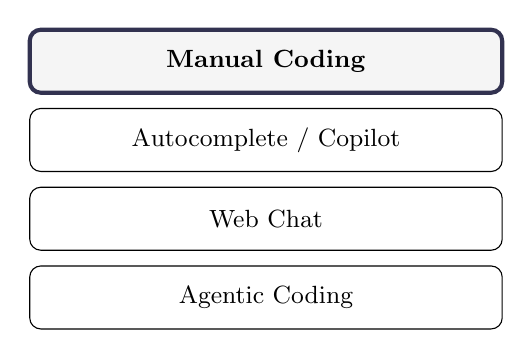
\begin{tikzpicture}[
        every node/.style={draw, rounded corners, minimum width=6cm, minimum height=0.8cm, align=center, font=\small}
      ]
        \node[fill=lightgray, draw=anthropic, line width=1.5pt] (manual) at (0,3.0) {\textbf{Manual Coding}};
        \node (copilot) at (0,2.0) {Autocomplete / Copilot};
        \node (chat) at (0,1.0) {Web Chat};
        \node (agentic) at (0,0) {Agentic Coding};
      \end{tikzpicture}

      \vspace{1em}
      You write every line. Full control, no assistance.

      \vspace{0.5em}
      This is what you do now in Stata or R.
    \end{column}
    \begin{column}{0.52\textwidth}
      \vspace{0.5em}
      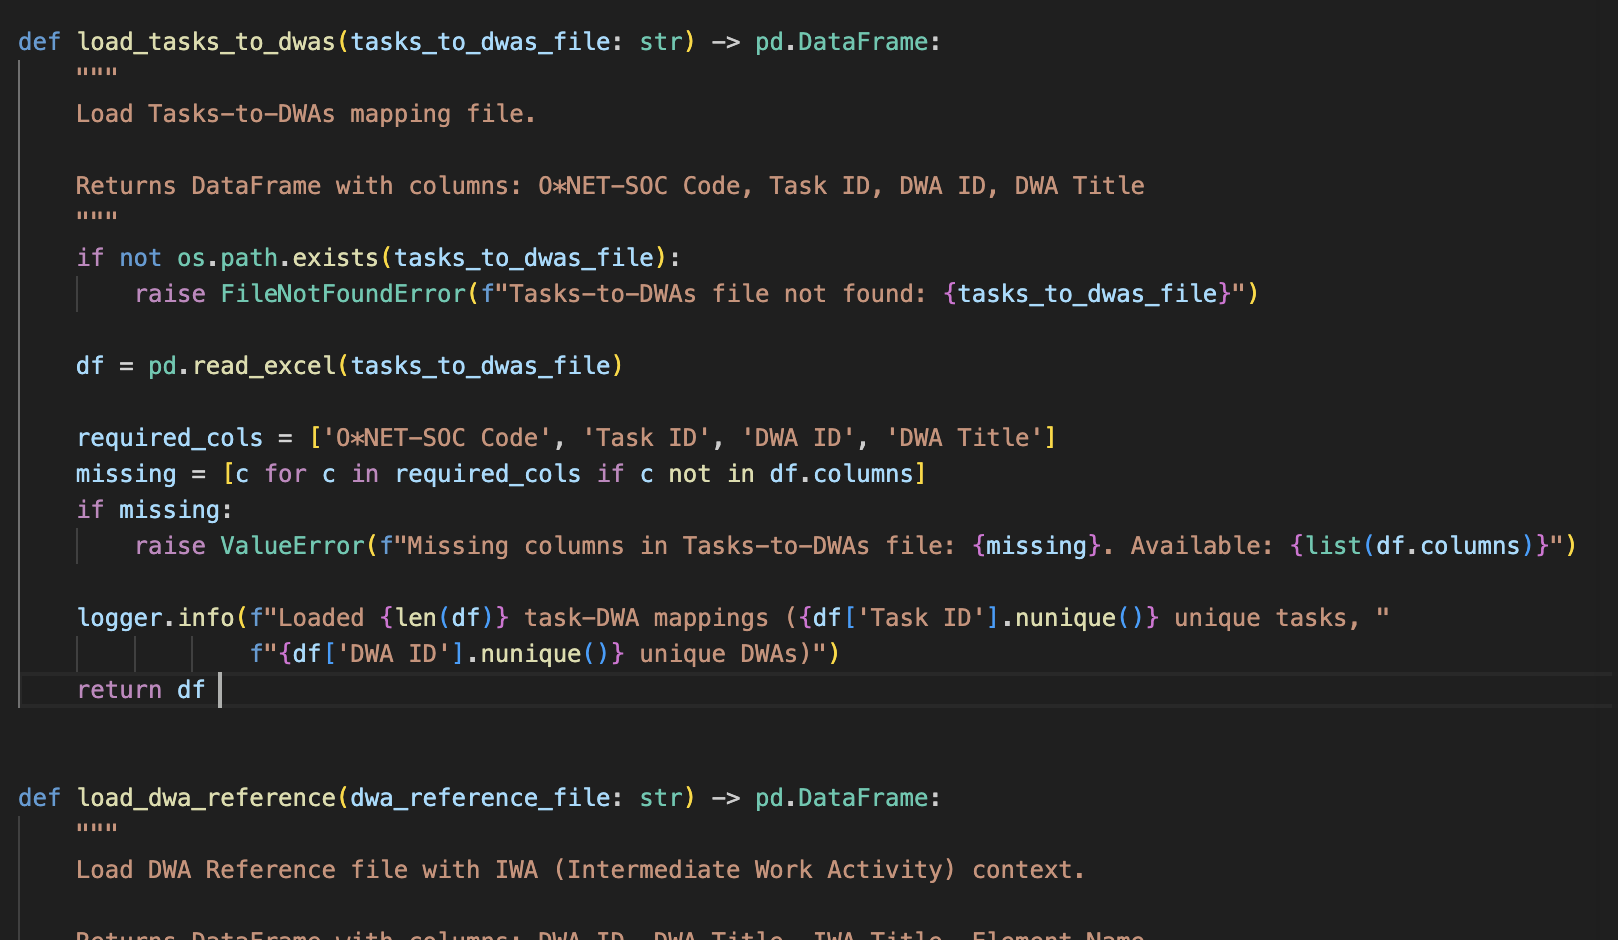
\includegraphics[width=\textwidth]{img/manual_coding.png}
    \end{column}
  \end{columns}
\end{frame}

% --- Paradigm 2: Copilot ---
\begin{frame}{The Coding Paradigm Spectrum: Autocomplete / Copilot}
  \begin{columns}[T]
    \begin{column}{0.45\textwidth}
      \vspace{0.5em}
      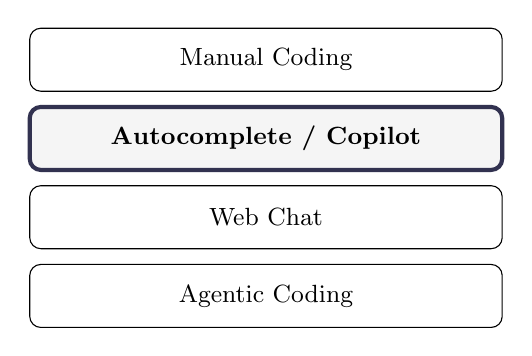
\begin{tikzpicture}[
        every node/.style={draw, rounded corners, minimum width=6cm, minimum height=0.8cm, align=center, font=\small}
      ]
        \node (manual) at (0,3.0) {Manual Coding};
        \node[fill=lightgray, draw=anthropic, line width=1.5pt] (copilot) at (0,2.0) {\textbf{Autocomplete / Copilot}};
        \node (chat) at (0,1.0) {Web Chat};
        \node (agentic) at (0,0) {Agentic Coding};
      \end{tikzpicture}

      \vspace{1em}
      AI suggests the next line as you type.

      \vspace{0.5em}
      You accept or reject. The AI assists; you drive.
    \end{column}
    \begin{column}{0.52\textwidth}
      \vspace{0.5em}
      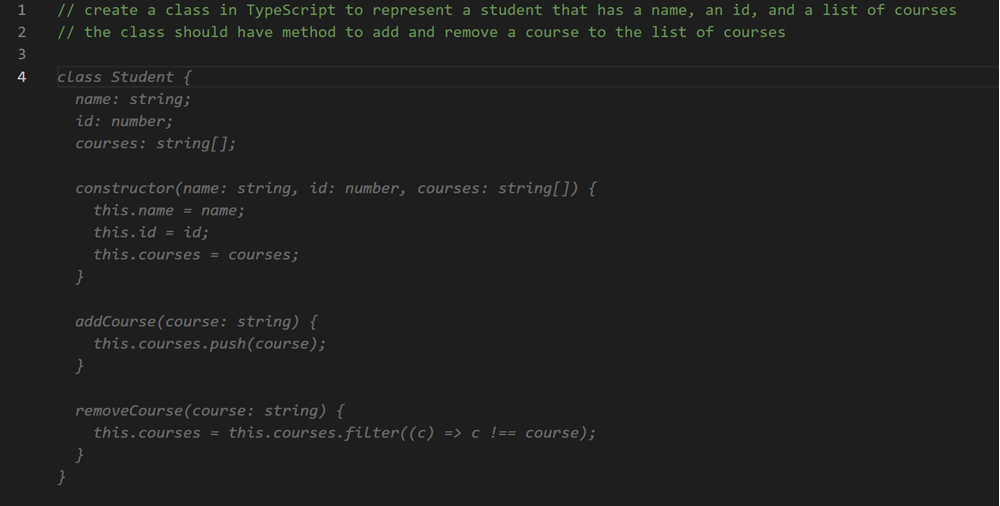
\includegraphics[width=\textwidth]{img/copilot.png}
    \end{column}
  \end{columns}
\end{frame}

% --- Paradigm 3: Web Chat ---
\begin{frame}{The Coding Paradigm Spectrum: Web Chat}
  \begin{columns}[T]
    \begin{column}{0.45\textwidth}
      \vspace{0.5em}
      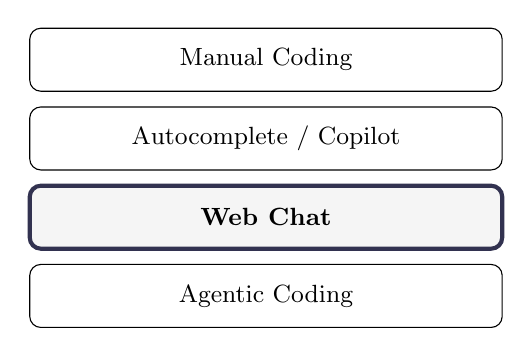
\begin{tikzpicture}[
        every node/.style={draw, rounded corners, minimum width=6cm, minimum height=0.8cm, align=center, font=\small}
      ]
        \node (manual) at (0,3.0) {Manual Coding};
        \node (copilot) at (0,2.0) {Autocomplete / Copilot};
        \node[fill=lightgray, draw=anthropic, line width=1.5pt] (chat) at (0,1.0) {\textbf{Web Chat}};
        \node (agentic) at (0,0) {Agentic Coding};
      \end{tikzpicture}

      \vspace{1em}
      You describe a task; AI gives you code to copy-paste.

      \vspace{0.5em}
      The AI cannot see your project.
    \end{column}
    \begin{column}{0.52\textwidth}
      \vspace{0.5em}
      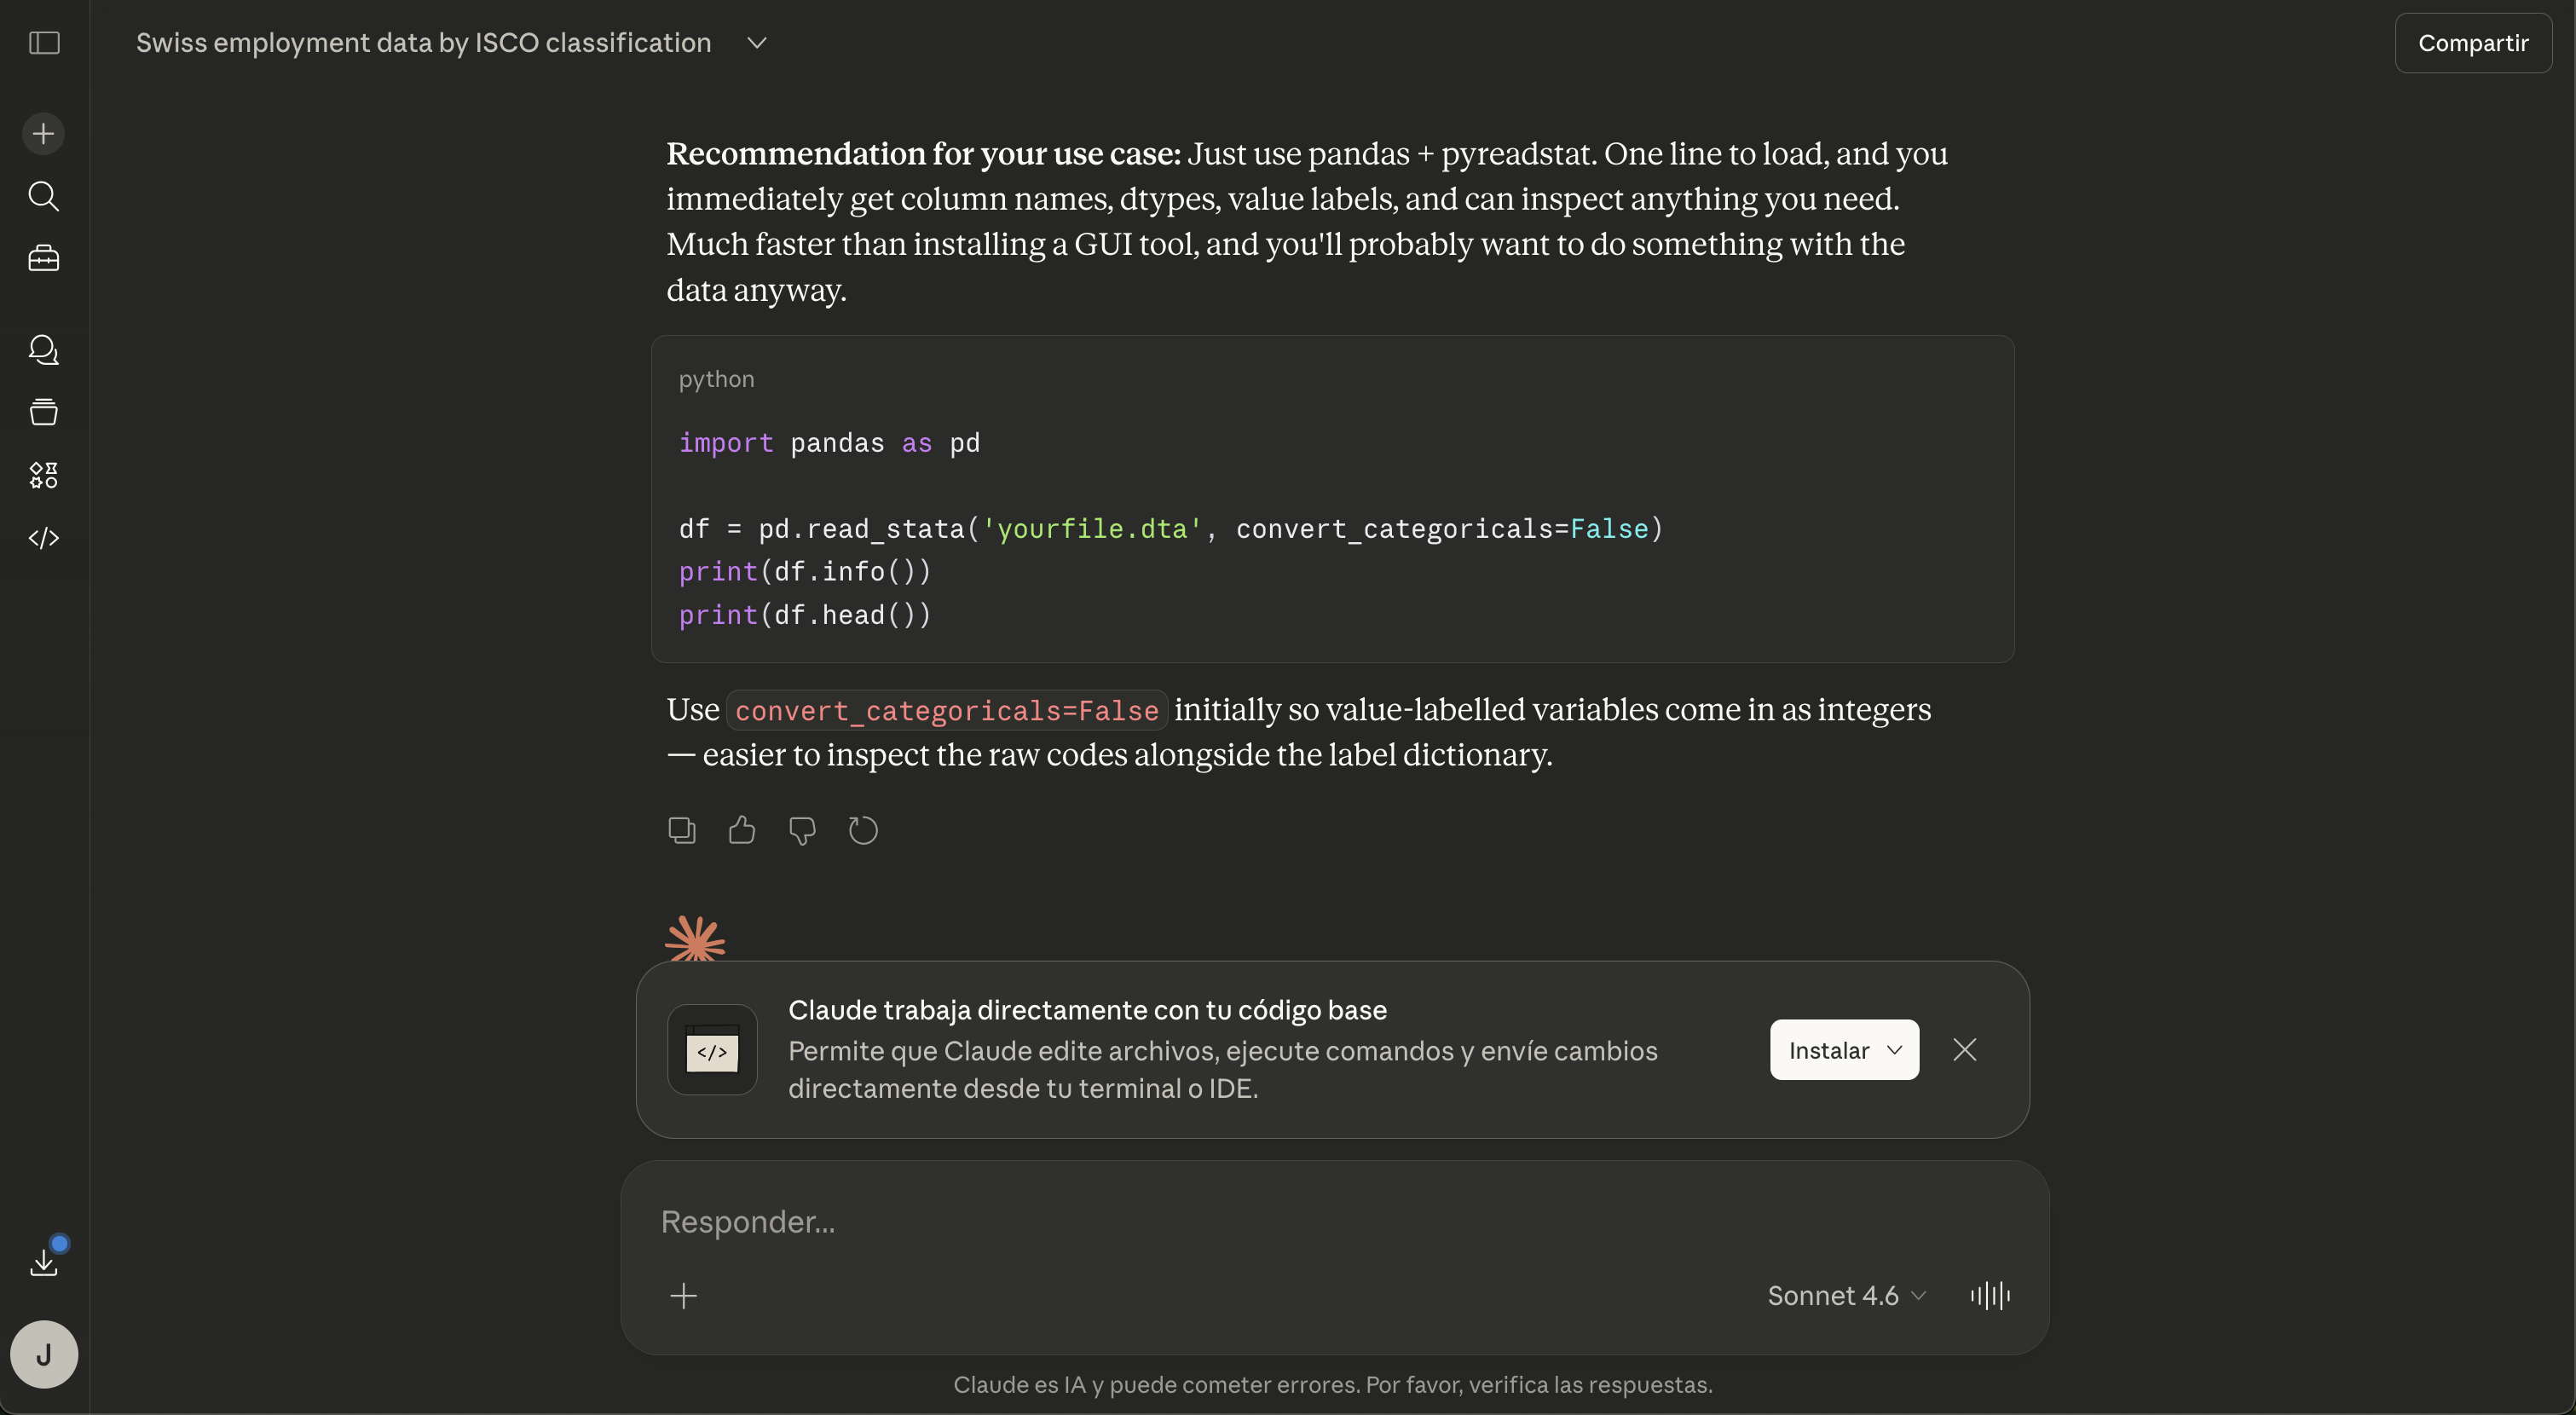
\includegraphics[width=\textwidth]{img/claude_web.png}
    \end{column}
  \end{columns}
\end{frame}

% --- Paradigm 4: Agentic Coding ---
\begin{frame}{The Coding Paradigm Spectrum: Agentic Coding}
  \begin{columns}[T]
    \begin{column}{0.45\textwidth}
      \vspace{0.5em}
      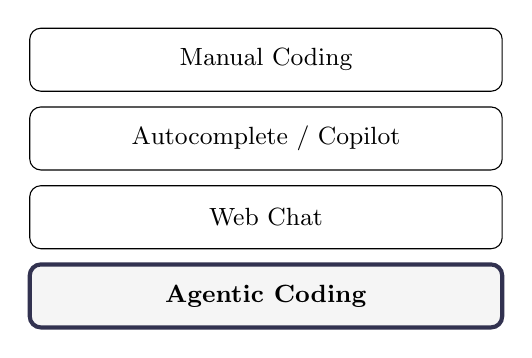
\begin{tikzpicture}[
        every node/.style={draw, rounded corners, minimum width=6cm, minimum height=0.8cm, align=center, font=\small}
      ]
        \node (manual) at (0,3.0) {Manual Coding};
        \node (copilot) at (0,2.0) {Autocomplete / Copilot};
        \node (chat) at (0,1.0) {Web Chat};
        \node[fill=lightgray, draw=anthropic, line width=1.5pt] (agentic) at (0,0) {\textbf{Agentic Coding}};
      \end{tikzpicture}

      \vspace{1em}
      AI reads, writes, and runs code \textbf{in your project}.
    \end{column}
    \begin{column}{0.52\textwidth}
      \vspace{0.5em}
      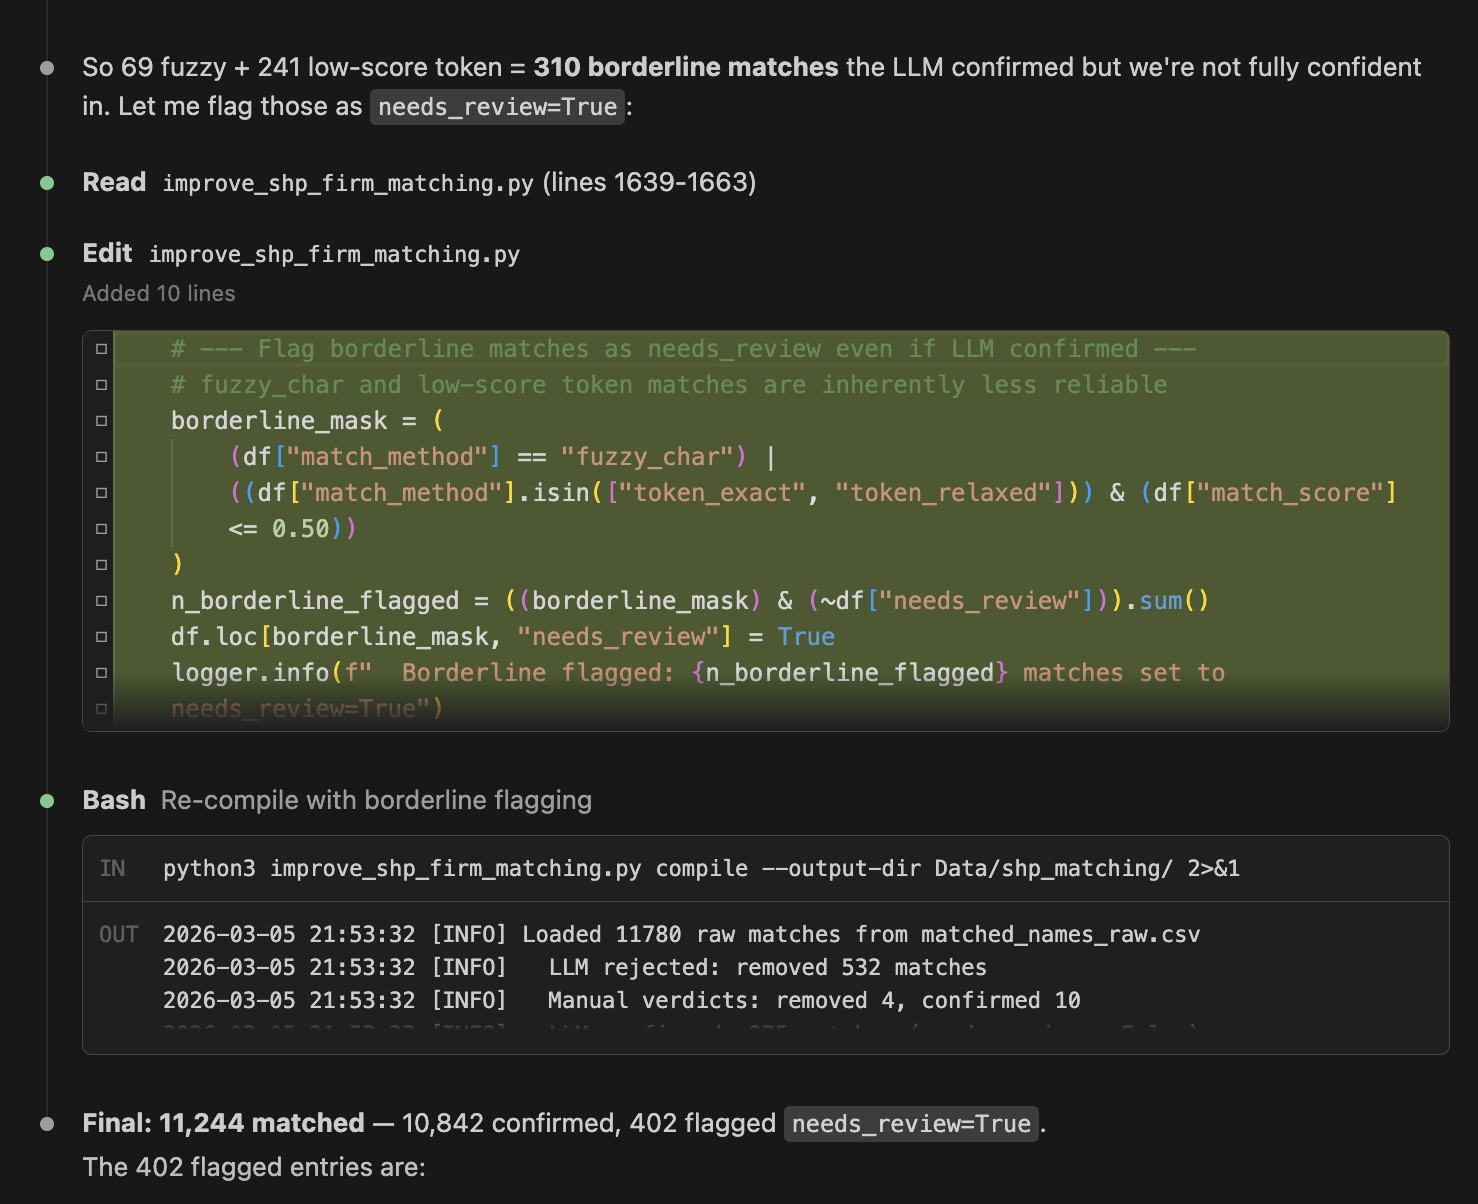
\includegraphics[width=\textwidth]{img/agentic_coding.png}
    \end{column}
  \end{columns}
\end{frame}

\begin{frame}{Why Agentic Coding Is Different}
  \small
  \begin{tabular}{@{}l l l@{}}
    \toprule
    \textbf{Paradigm} & \textbf{Pros} & \textbf{Cons} \\
    \midrule
    Manual Coding & Full control & Slow, everything by hand \\
    Autocomplete / Copilot & You control logic and structure & Still line-by-line \\
    Web Chat & Can handle complex tasks & Copy-paste; AI misses context \\
    \textbf{Agentic Coding} & \textbf{Fastest; works on your project} & \textbf{Can act autonomously} \\
    \bottomrule
  \end{tabular}

  \vspace{0.8em}
  \begin{alertblock}{The Key Insight}
    Agentic coding is the first paradigm where the tool \textbf{interacts with your project directly and autonomously}.
    That is what makes it so productive, and why learning to use it well matters.
  \end{alertblock}

  \vspace{0.3em}
  These principles apply to Claude Code, Cursor, Codex, Windsurf, or whatever comes next.
\end{frame}

% ══════════════════════════════════════════════════════════════════
%  WHAT IT CAN AND CANNOT DO  [16:00–19:00]
% ══════════════════════════════════════════════════════════════════

\begin{frame}{What Claude Code Can Do for Academic Research}
  \footnotesize
  \begin{columns}[T]
    \begin{column}{0.48\textwidth}
      \textbf{Data Work}
      \begin{itemize}
        \item Clean, reshape, and merge datasets
        \item Construct variables from raw data
        \item Build panel datasets across sources
        \item Handle missing data, recoding, harmonization
      \end{itemize}

      \vspace{0.5em}
      \textbf{Analysis}
      \begin{itemize}
        \item Exploratory data analysis and summary statistics
        \item Generate robustness checks and specification variants
        \item Create publication-quality visualizations
        \item Synthesize results across specifications
      \end{itemize}
    \end{column}
    \begin{column}{0.48\textwidth}
      \textbf{Writing and Review}
      \begin{itemize}
        \item Draft methods sections, data descriptions, results summaries
        \item Audit existing scripts for silent errors
        \item Review code against your methods section
        \item Write documentation, READMEs, replication packages
      \end{itemize}

      \vspace{0.5em}
      \textbf{Research Infrastructure}
      \begin{itemize}
        \item Process text corpora at scale (NLP, classification)
        \item Web scraping and API data collection
        \item Crosswalk and linkage construction
        \item Refactor and optimize slow pipelines
      \end{itemize}
    \end{column}
  \end{columns}
\end{frame}

\begin{frame}{A Tool Built for Software Engineers}
  Claude Code was designed for professional developers. Their world is different from ours.

  \vspace{0.5em}
  \begin{columns}[T]
    \begin{column}{0.48\textwidth}
      \textbf{Software Engineering}
      \begin{itemize}
        \item ``Works'' = \textbf{runs correctly}. Clear success criteria: tests pass, feature ships, users are happy
        \item Code is the product
        \item Errors are caught by automated tests
        \item Speed and iteration are paramount
      \end{itemize}
    \end{column}
    \begin{column}{0.48\textwidth}
      \textbf{Academic Research}
      \begin{itemize}
        \item ``Works'' = \textbf{???}. Code that runs without errors can produce completely wrong results. Output that looks plausible can be based on the wrong sample, wrong specification, or wrong variable
        \item Code is the \textit{instrument}; the paper is the product
        \item Errors are caught by \textit{you}, or by Reviewer 2
        \item Correctness matters more than speed
      \end{itemize}
    \end{column}
  \end{columns}

  \vspace{0.5em}
  The defaults, instincts, and shortcuts built into these tools reflect engineering priorities.\\
  \textbf{Using them well for research means overriding some of those defaults.}
\end{frame}

\begin{frame}{Do You Own It?}
  \begin{block}{}
    Pick any result your code produced. Without looking at the code:\\
    what got dropped, what got merged, and why?
  \end{block}

  \vspace{0.3em}
  If you can't answer that in 30 seconds, you don't own it.

  \vspace{0.5em}
  \textbf{Before you delegate:}
  \begin{itemize}
    \item What would wrong look like? Can I describe a specific failure mode before I run this?
  \end{itemize}

  \vspace{0.3em}
  \textbf{After you delegate:}
  \begin{itemize}
    \item Can I describe what this code does without reading it?
    \item Can I state what decisions shaped the output and why?
  \end{itemize}

  \vspace{0.5em}
  You didn't write it. That's fine.\\
  But every decision in it is yours. \textbf{Can you justify it as if you chose it yourself?}
\end{frame}

% ══════════════════════════════════════════════════════════════════
%  WHY VERIFICATION MATTERS  [19:00–23:00]
% ══════════════════════════════════════════════════════════════════

\begin{frame}{Why Verification Matters}
  {\large What happens when you skip verification:}

  \vspace{0.8em}
  \begin{enumerate}
    \item \textbf{Silent observation loss:} A merge silently drops 300 observations.\\
      The code looks clean. The error is invisible without checking row counts.

      \vspace{0.5em}
    \item \textbf{Invalid transformation:} A log transformation applied to a variable containing zeros.\\
      No error raised, wrong results.

      \vspace{0.5em}
    \item \textbf{Incorrect panel operations:} A lagged variable computed without sorting by time within panels.
  \end{enumerate}

  \vspace{0.5em}
  \alert{These are the kinds of errors that end up in published work.}
\end{frame}

% ══════════════════════════════════════════════════════════════════
%  THE CONTROL PRINCIPLE  [23:00–25:00]
% ══════════════════════════════════════════════════════════════════

\begin{frame}{The Control Principle}
  \begin{alertblock}{You Are the PI. Claude Code Is the RA.}
    The question is not ``can Claude Code do this'' but\\
    ``what is the best way to get this done reliably.''
  \end{alertblock}

  \vspace{1em}
  \centering
  \textbf{If you cannot verify a result, you should not delegate the task.}

\end{frame}

% ══════════════════════════════════════════════════════════════════
%  WHY PYTHON  [25:00–27:00]
% ══════════════════════════════════════════════════════════════════

\begin{frame}{Why Python}
  \begin{columns}[T]
    \begin{column}{0.48\textwidth}
      \begin{itemize}
        \item Claude Code is substantially better at Python than Stata or R
        \item The principles (task decomposition, verification, control) transfer to any language
        \item Python is increasingly where the tools and ecosystem are for computational research
      \end{itemize}
    \end{column}
    \begin{column}{0.48\textwidth}
      \vspace{0.3em}
      
\includegraphics[width=\textwidth]{img/python_vs_r.png}
    \end{column}
  \end{columns}
\end{frame}

% ══════════════════════════════════════════════════════════════════
%  ORIENTATION: TERMINAL, VS CODE, FILE TYPES  [27:00–37:00]
% ══════════════════════════════════════════════════════════════════

\begin{frame}{Where Does Claude Code Live?}
  \begin{columns}[T]
    \begin{column}{0.55\textwidth}
      Claude Code runs \textbf{inside your terminal}, not in a browser, not in an app.

      \vspace{0.5em}
      \begin{enumerate}
        \item You open a terminal
        \item Navigate to your project: \lstinline{cd my_project/}
        \item Type \lstinline{claude} and press Enter
        \item You're now talking to Claude Code
      \end{enumerate}

      \vspace{0.5em}
      It can see your files, read your data, write scripts, and run them, all without copying and pasting.
    \end{column}
    \begin{column}{0.42\textwidth}
      \vspace{0.3em}
      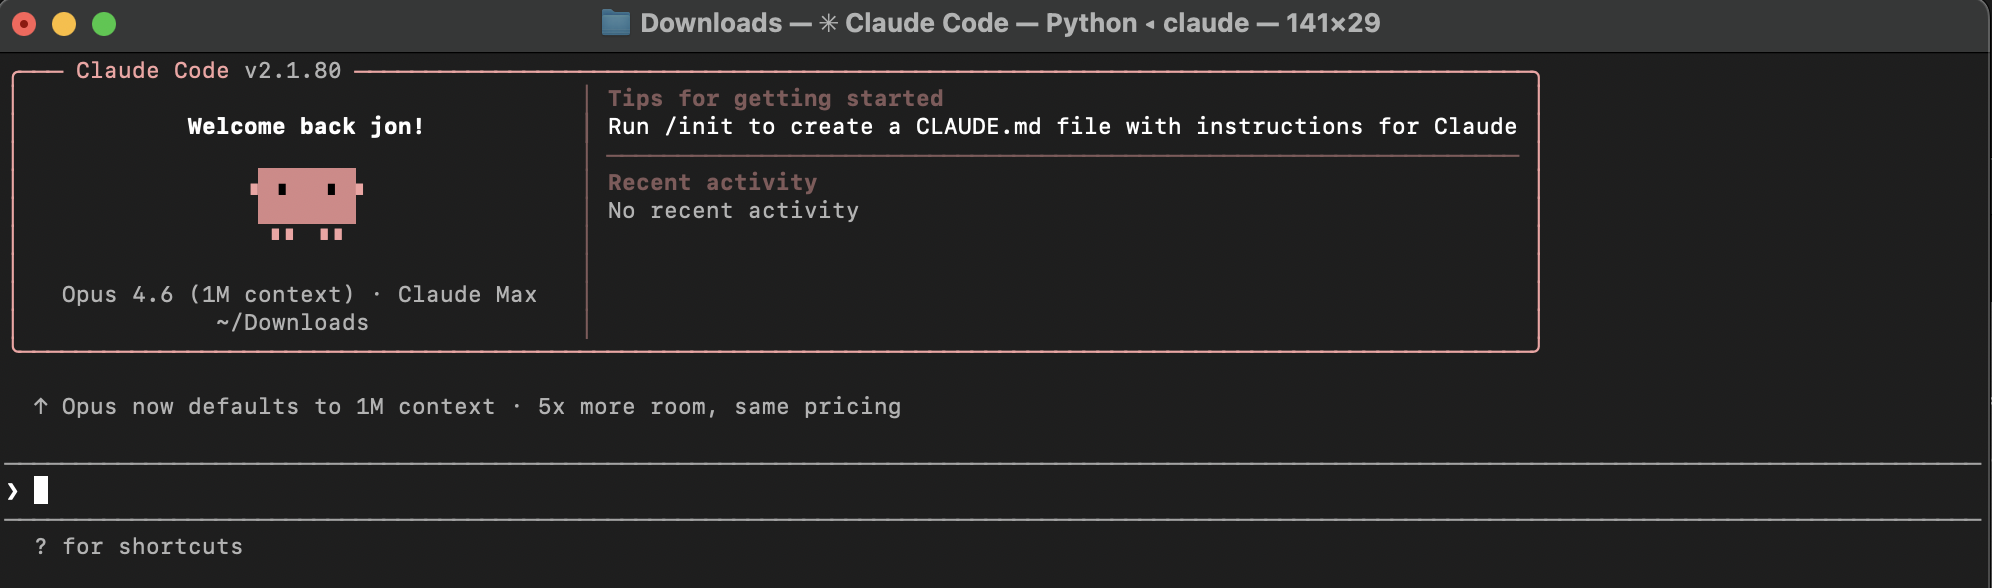
\includegraphics[width=\textwidth]{img/claude_code_terminal.png}

      \vspace{0.3em}
      {\footnotesize\textit{This is what Claude Code looks like when you launch it.}}
    \end{column}
  \end{columns}
\end{frame}

\begin{frame}[fragile]{What Is the Terminal?}
  \textbf{The terminal} is a text-based interface to your computer. Instead of clicking, you type commands.

  \vspace{0.3em}
  \begin{columns}[T]
    \begin{column}{0.42\textwidth}
      \vspace{0.3em}
      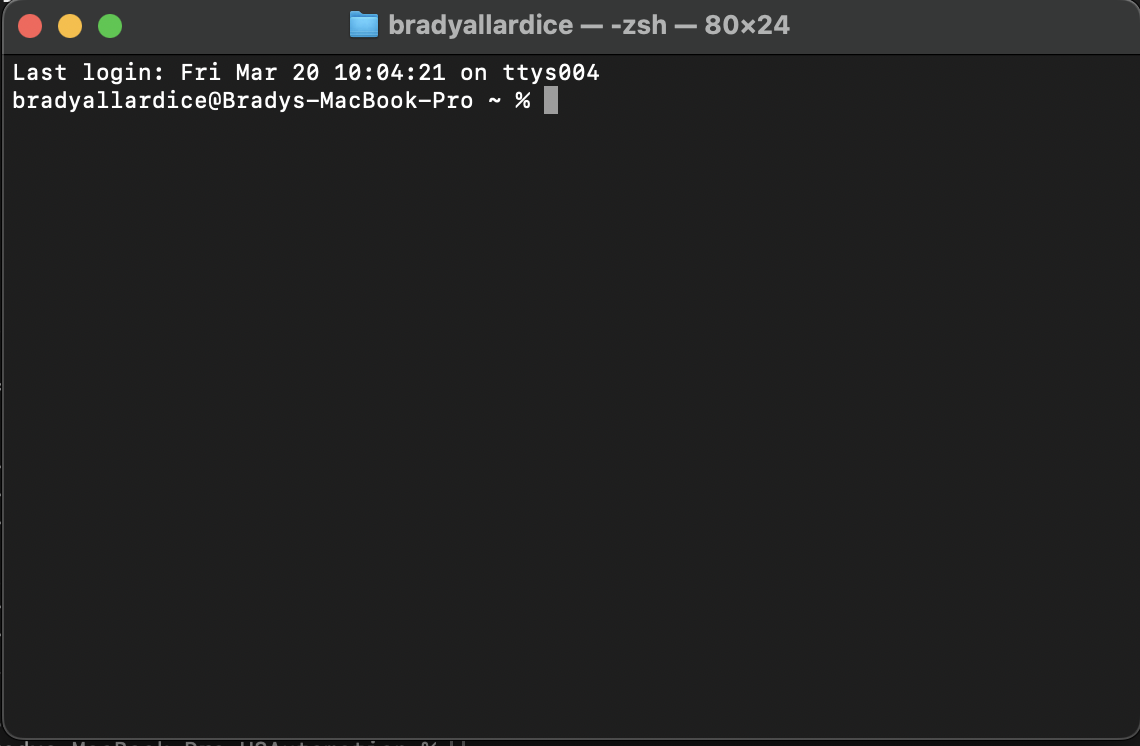
\includegraphics[width=\textwidth]{img/terminal.png}
      {\footnotesize\textit{Claude Code writing and running code in the terminal.}}
    \end{column}
    \begin{column}{0.54\textwidth}
      \textbf{Essential commands:}
      \vspace{0.2em}
\begin{lstlisting}
# Where am I?
pwd

# What's in this folder?
ls

# Move into a folder
cd my_project/

# Run a Python script
python my_script.py

# Launch Claude Code
claude
\end{lstlisting}
      \vspace{0.2em}
      {\small You may hear it called: terminal, command line, shell, console. All roughly the same thing.}
    \end{column}
  \end{columns}
\end{frame}

% ── Where Claude Code Runs: Surfaces ─────────────────────────────
\begin{frame}{Same Claude Code, Different Front Doors}
  \small
  Claude Code is \textbf{one agent}. You can reach it from several places, and it behaves the same in all of them:

  \vspace{0.4em}
  \begin{tabular}{@{}p{0.27\textwidth} p{0.66\textwidth}@{}}
    \toprule
    \textbf{Where} & \textbf{What it is / when to use it} \\
    \midrule
    \textbf{Terminal (CLI)} & The original. Run \lstinline{claude} in any project folder --- full agent, always available, great for quick jobs or tools without an editor plug-in. \\[0.3em]
    \textbf{VS Code / JetBrains} & \textbf{Our home base for this course.} The same agent inside your editor: inline diffs, click-to-open file references, your code and Claude side by side. \\[0.3em]
    \textbf{Desktop app} & Claude Code in its own window (Mac/Windows) instead of a terminal. \\[0.3em]
    \textbf{Web (claude.ai/code)} & Claude Code in the browser for cloud sessions --- nothing to install. \\
    \bottomrule
  \end{tabular}

  \vspace{0.5em}
  \begin{alertblock}{Not the same as the Claude app}
    The \textbf{Claude app} (claude.ai or the desktop chat) is a conversational assistant: you paste text in and copy answers out. It can't see your project, run your code, or edit files in place. \textbf{Claude Code} acts directly in your repo --- reading files, editing them, and running commands for you.
  \end{alertblock}
\end{frame}

% ── Terminal Example: Editing a Document ─────────────────────────
\begin{frame}[fragile]{Terminal Example: Editing a Document}
  The terminal isn't just for code. Open Claude Code in any folder and ask it to edit a document --- notes, a README, a draft.

  \vspace{0.4em}
\begin{lstlisting}
cd ~/my_workspace/session_1
claude
\end{lstlisting}

  \vspace{0.3em}
  Then ask, in plain language:
\begin{lstlisting}[basicstyle=\ttfamily\footnotesize]
> Open notes.md and tighten the Summary section
  to three bullet points. Keep my wording where
  you can, and don't touch the other sections.
\end{lstlisting}

  \vspace{0.3em}
  Claude reads the file, shows a \textbf{proposed diff}, and waits for you to \textbf{approve, reject, or ask for changes} --- the same review loop you'll use everywhere.
\end{frame}

\begin{frame}{Terminal vs.\ VS Code}
  \textbf{The terminal} is how you'd normally interact with Claude Code --- especially if you're working in \textbf{Stata}, where there isn't a tight editor integration.

  \vspace{0.6em}
  But for this course, we'll be working in \textbf{VS Code}: the file you're editing, the code Claude is writing, and the conversation all live in one window.
\end{frame}

\begin{frame}{Why VS Code?}
  \small
  \begin{columns}[T]
    \begin{column}{0.38\textwidth}
      \textbf{VS Code} is a free code editor with a built-in terminal.

      \vspace{0.3em}
      Everything in one window:
      \begin{itemize}
        \item \textbf{Left:} file explorer
        \item \textbf{Center:} your code
        \item \textbf{Right:} Claude Code
      \end{itemize}

      \vspace{0.3em}
      You see what Claude Code writes \textit{as it writes it}.

      \vspace{0.3em}
      Today we use three features:
      \begin{enumerate}
        \item Open a folder
        \item View files in the editor
        \item Talk to Claude Code
      \end{enumerate}
    \end{column}
    \begin{column}{0.59\textwidth}
      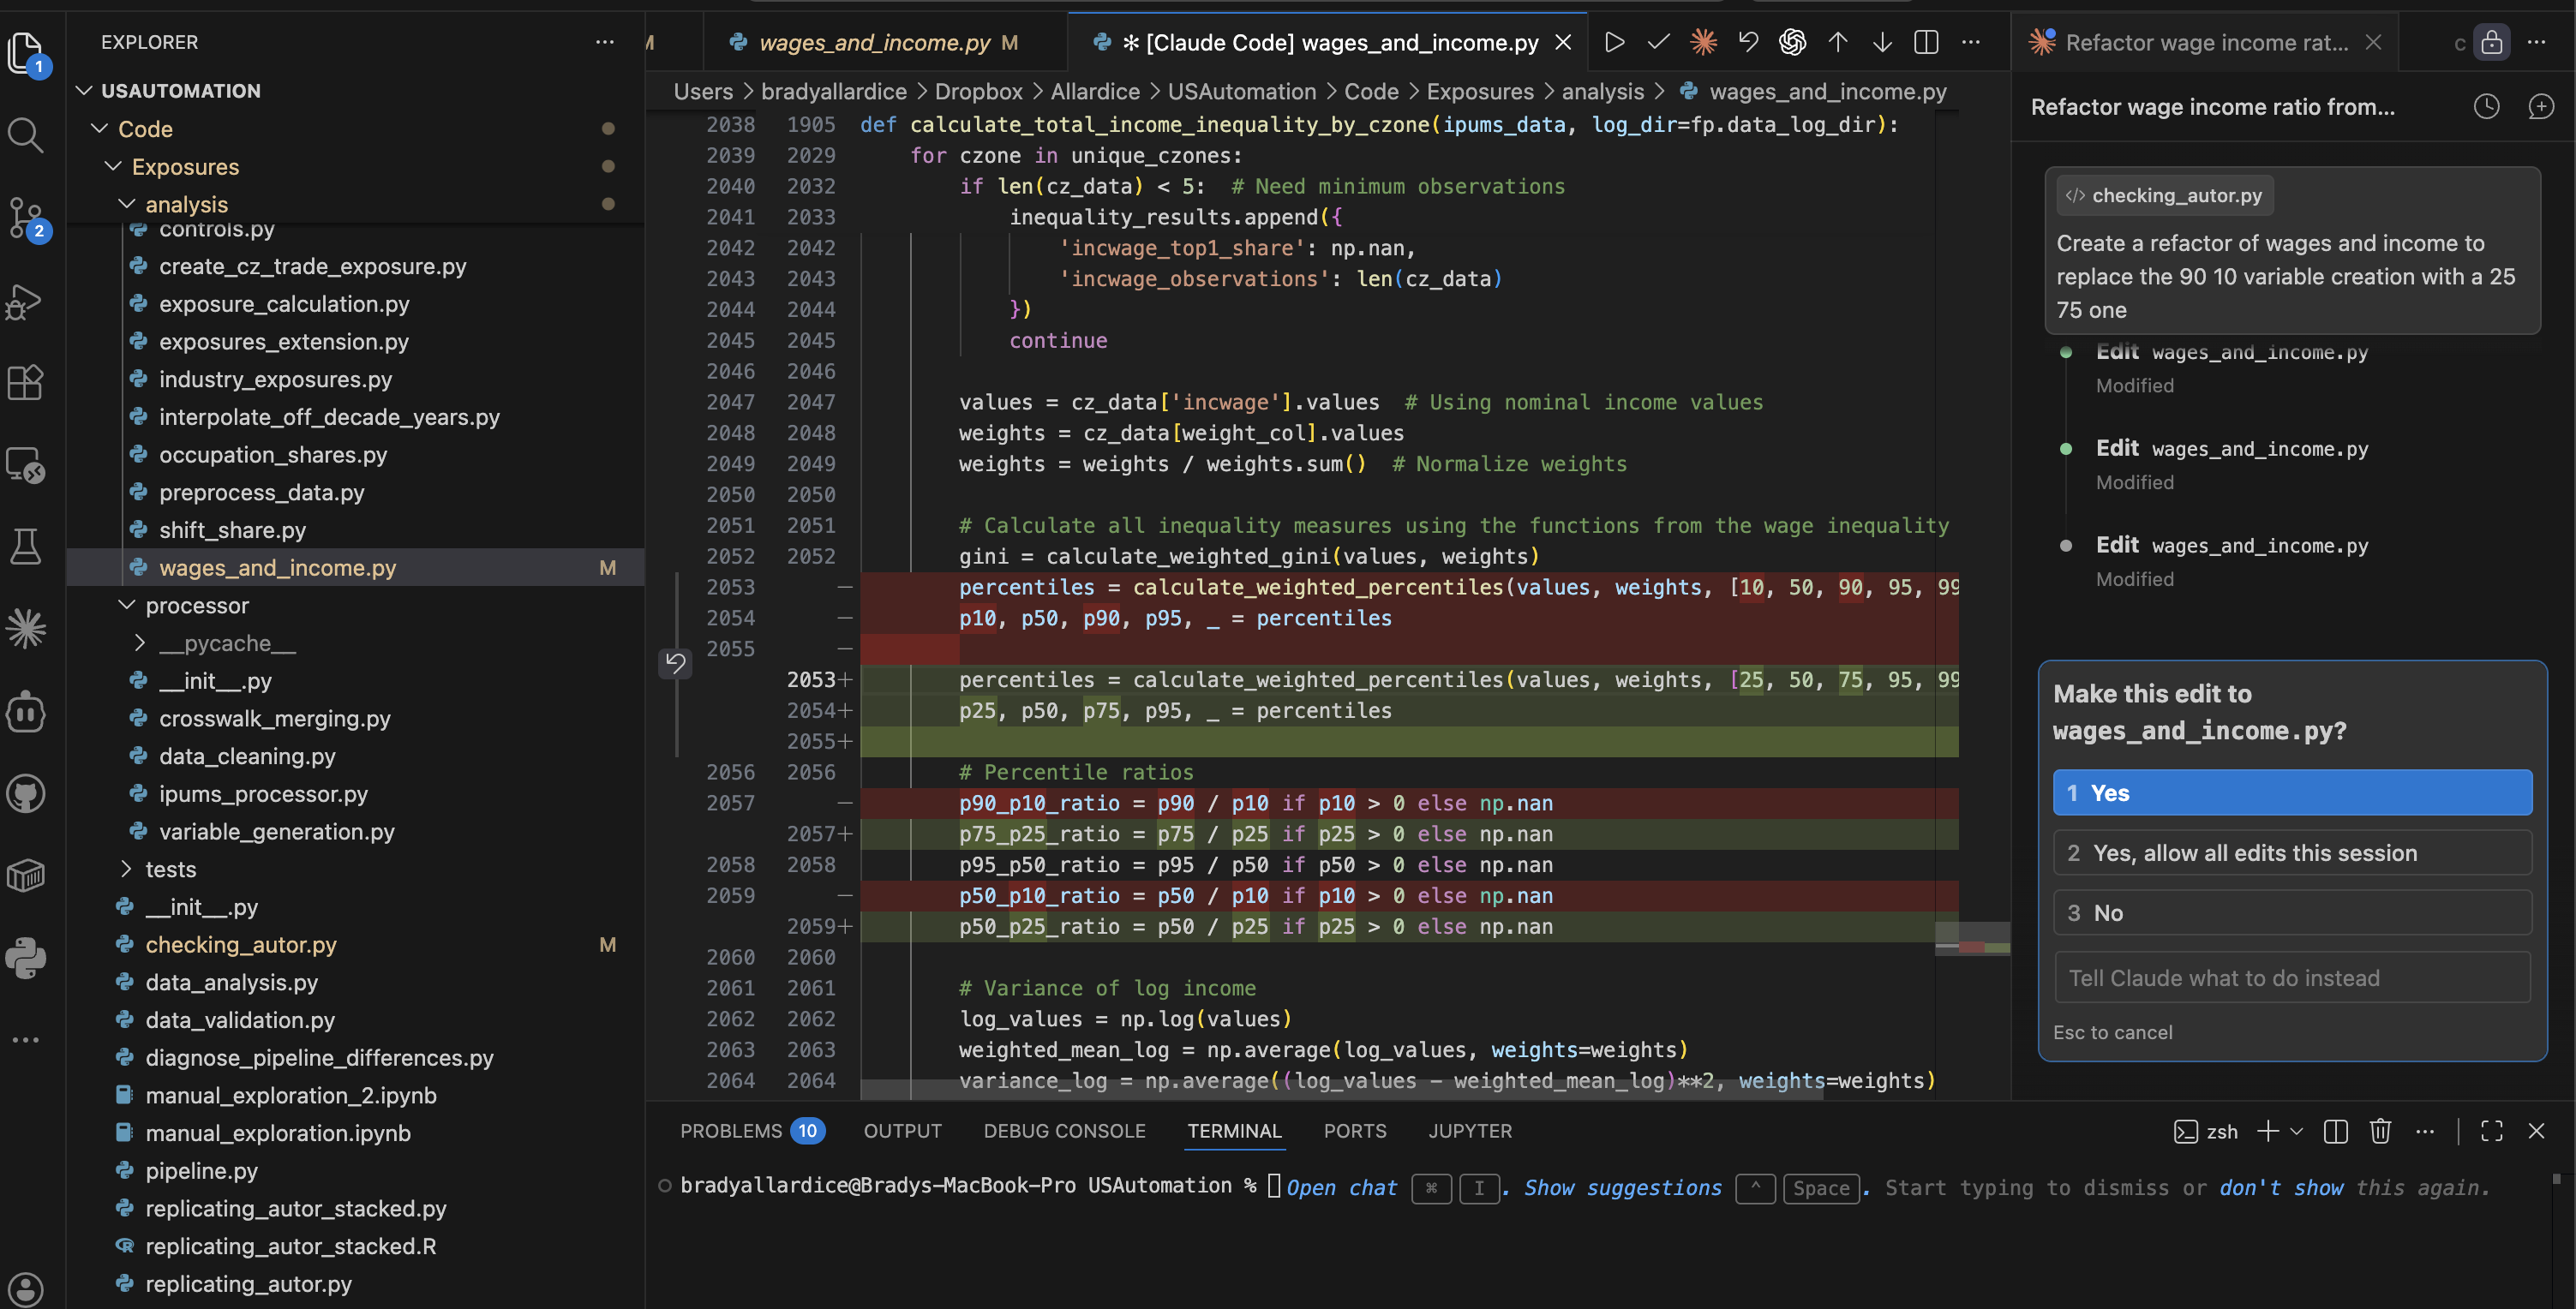
\includegraphics[width=\textwidth]{img/claude_mid_update.png}

      \vspace{0.2em}
      {\footnotesize Coming from RStudio? \href{https://www.youtube.com/watch?v=rKPfssR66GM}{\beamergotobutton{Configure VS Code to look like RStudio}}}
    \end{column}
  \end{columns}
\end{frame}

\begin{frame}{VS Code Runs Your Code Too}
  VS Code isn't just an editor --- with the right extensions, it executes your scripts directly:

  \vspace{0.4em}
  \begin{columns}[T]
    \begin{column}{0.54\textwidth}
      \begin{itemize}
        \item \textbf{Python} (\texttt{.py}, \texttt{.ipynb}) --- run line-by-line with Shift+Enter, or run the whole file
        \item \textbf{R} (\texttt{.R}, \texttt{.Rmd}) --- same workflow as RStudio, same interactive console
        \item \textbf{Stata} (\texttt{.do}) --- run do-files via the Stata extension, results in the integrated terminal
      \end{itemize}
    \end{column}
    \begin{column}{0.44\textwidth}
      
\includegraphics[width=\textwidth]{img/stata_extention.png}

      \vspace{0.2em}
      {\footnotesize\textit{The Stata extension for VS Code.}}
    \end{column}
  \end{columns}

  \vspace{0.4em}
  One editor, one window: Claude writes the code, and you run it without leaving the screen.
\end{frame}

\begin{frame}{Python Files: \texttt{.py} vs.\ \texttt{.ipynb}}
  \begin{columns}[T]
    \begin{column}{0.48\textwidth}
      \textbf{Notebooks} (\texttt{.ipynb})

      \vspace{0.3em}
      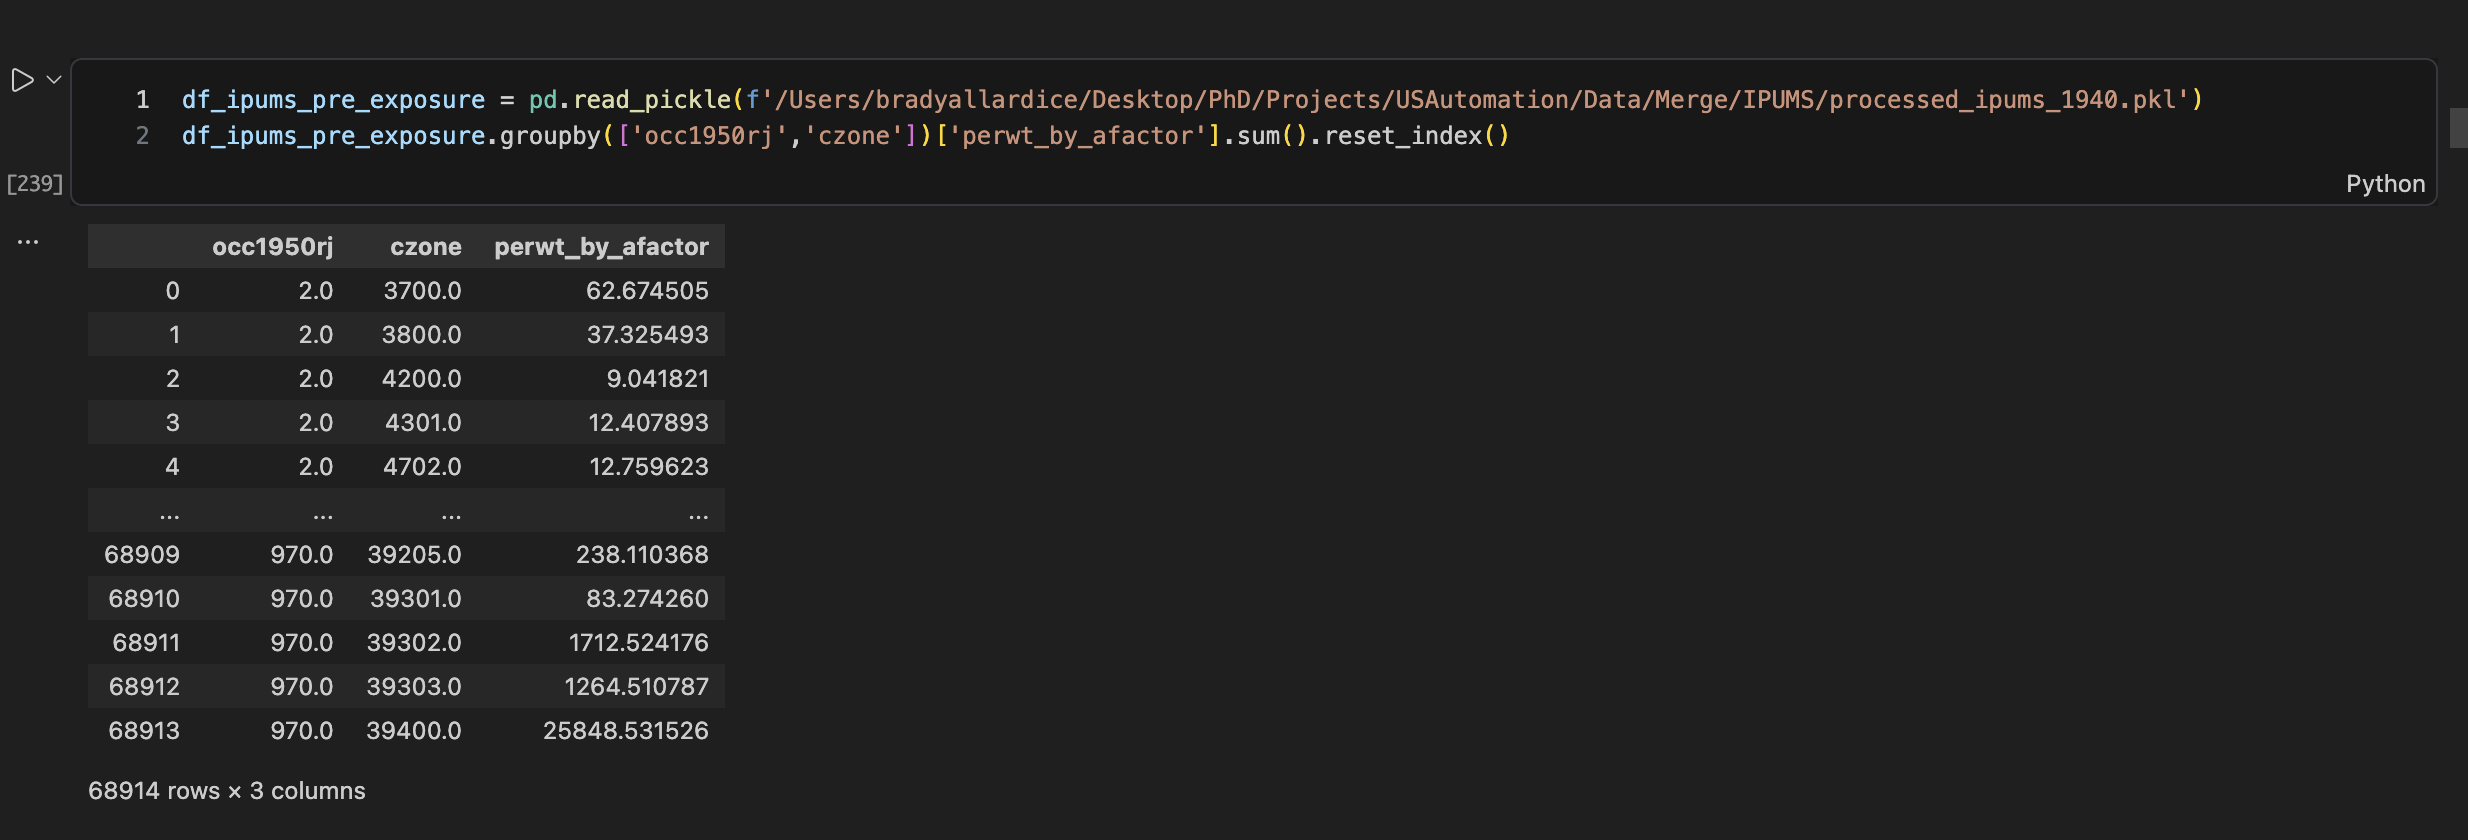
\includegraphics[width=\textwidth]{img/notebook_dataframe.png}

      \vspace{0.2em}
      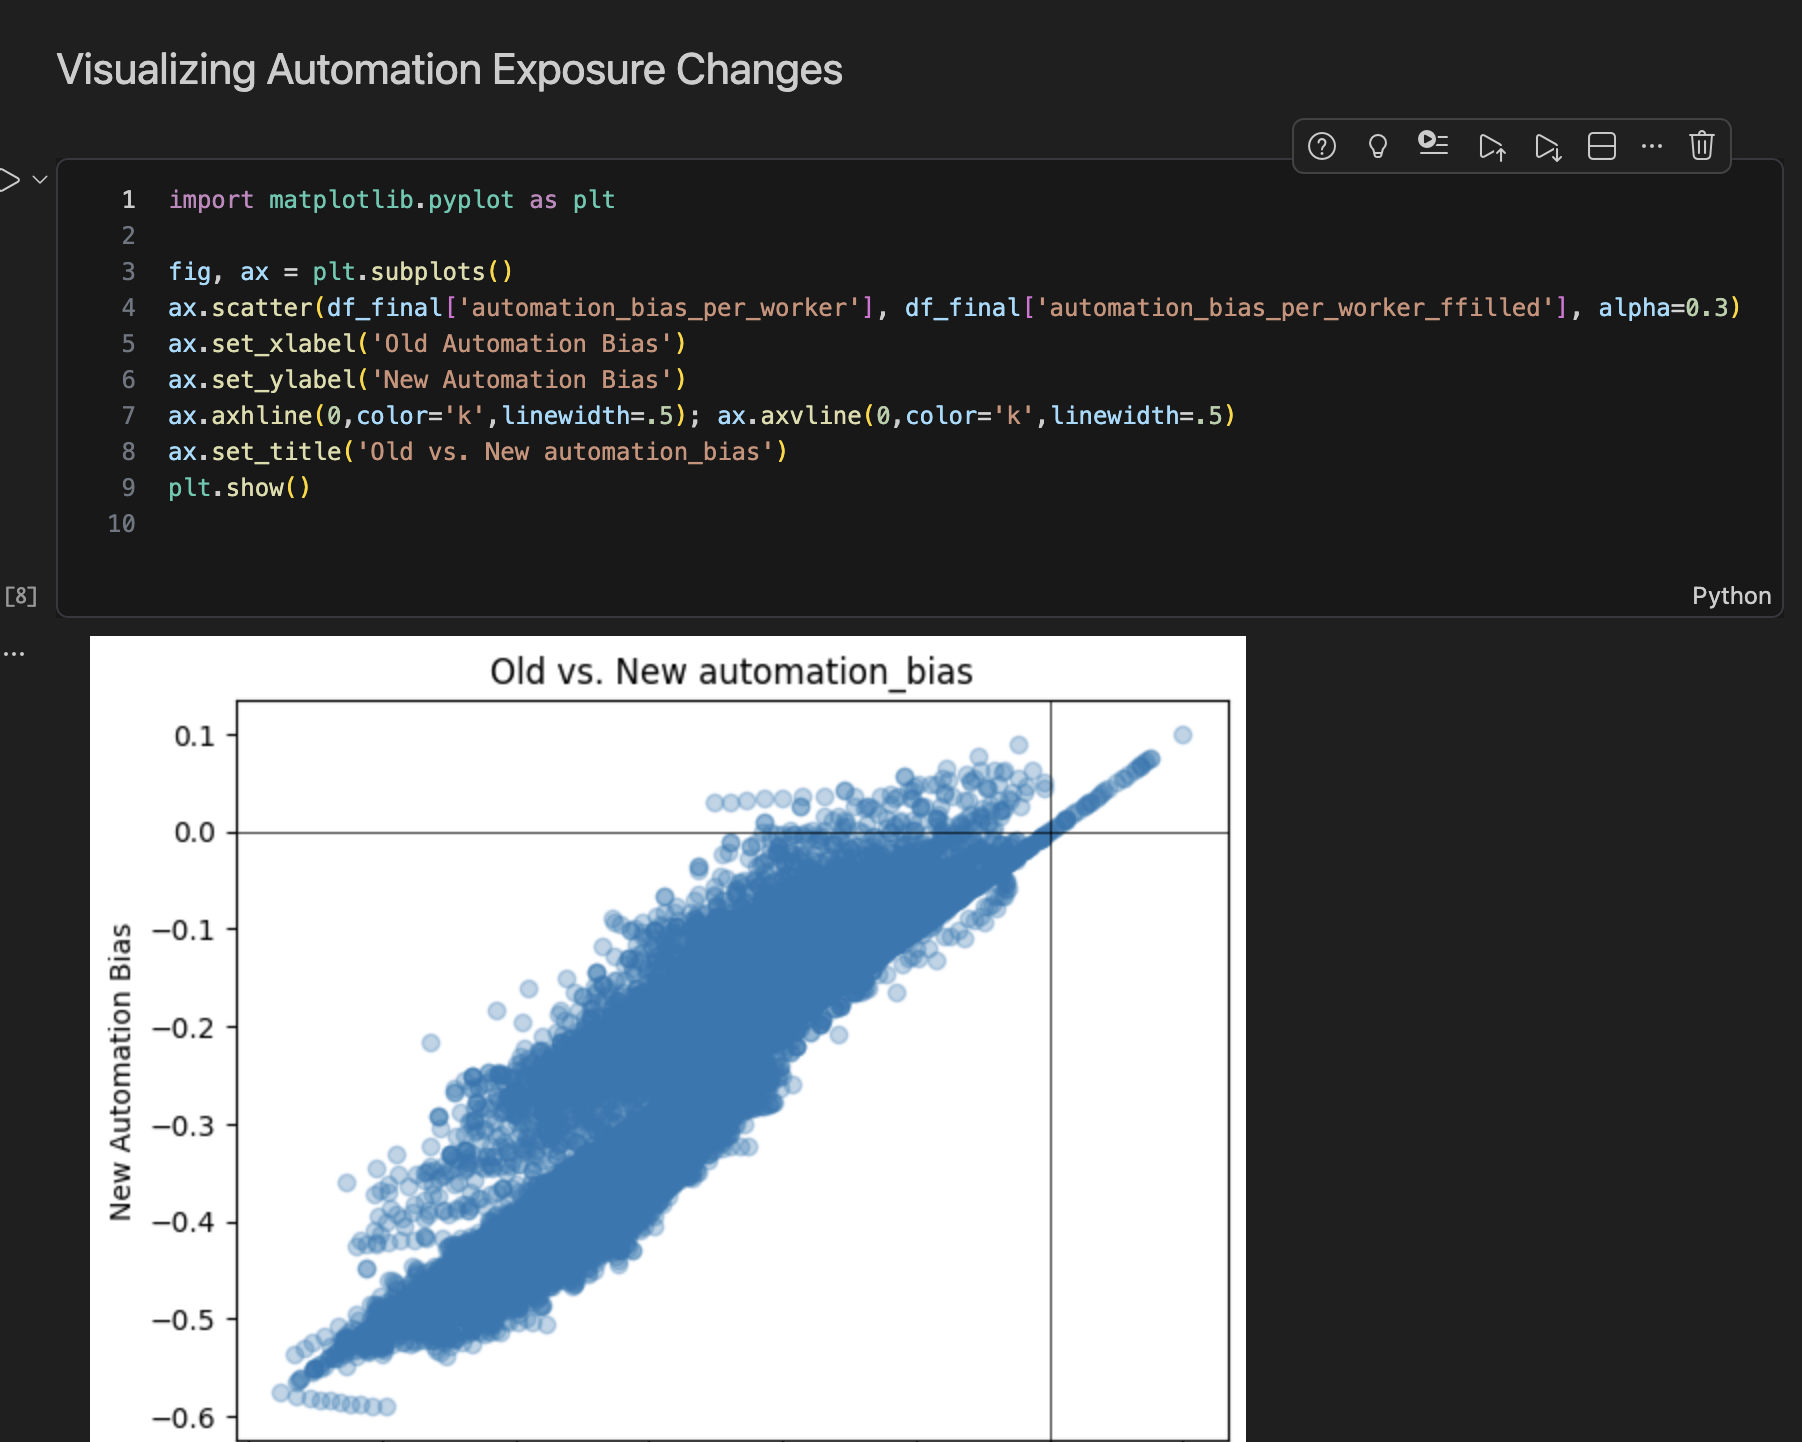
\includegraphics[width=0.7\textwidth]{img/notebook_example.png}
    \end{column}
    \begin{column}{0.48\textwidth}
      \textbf{Scripts} (\texttt{.py})

      \vspace{0.3em}
      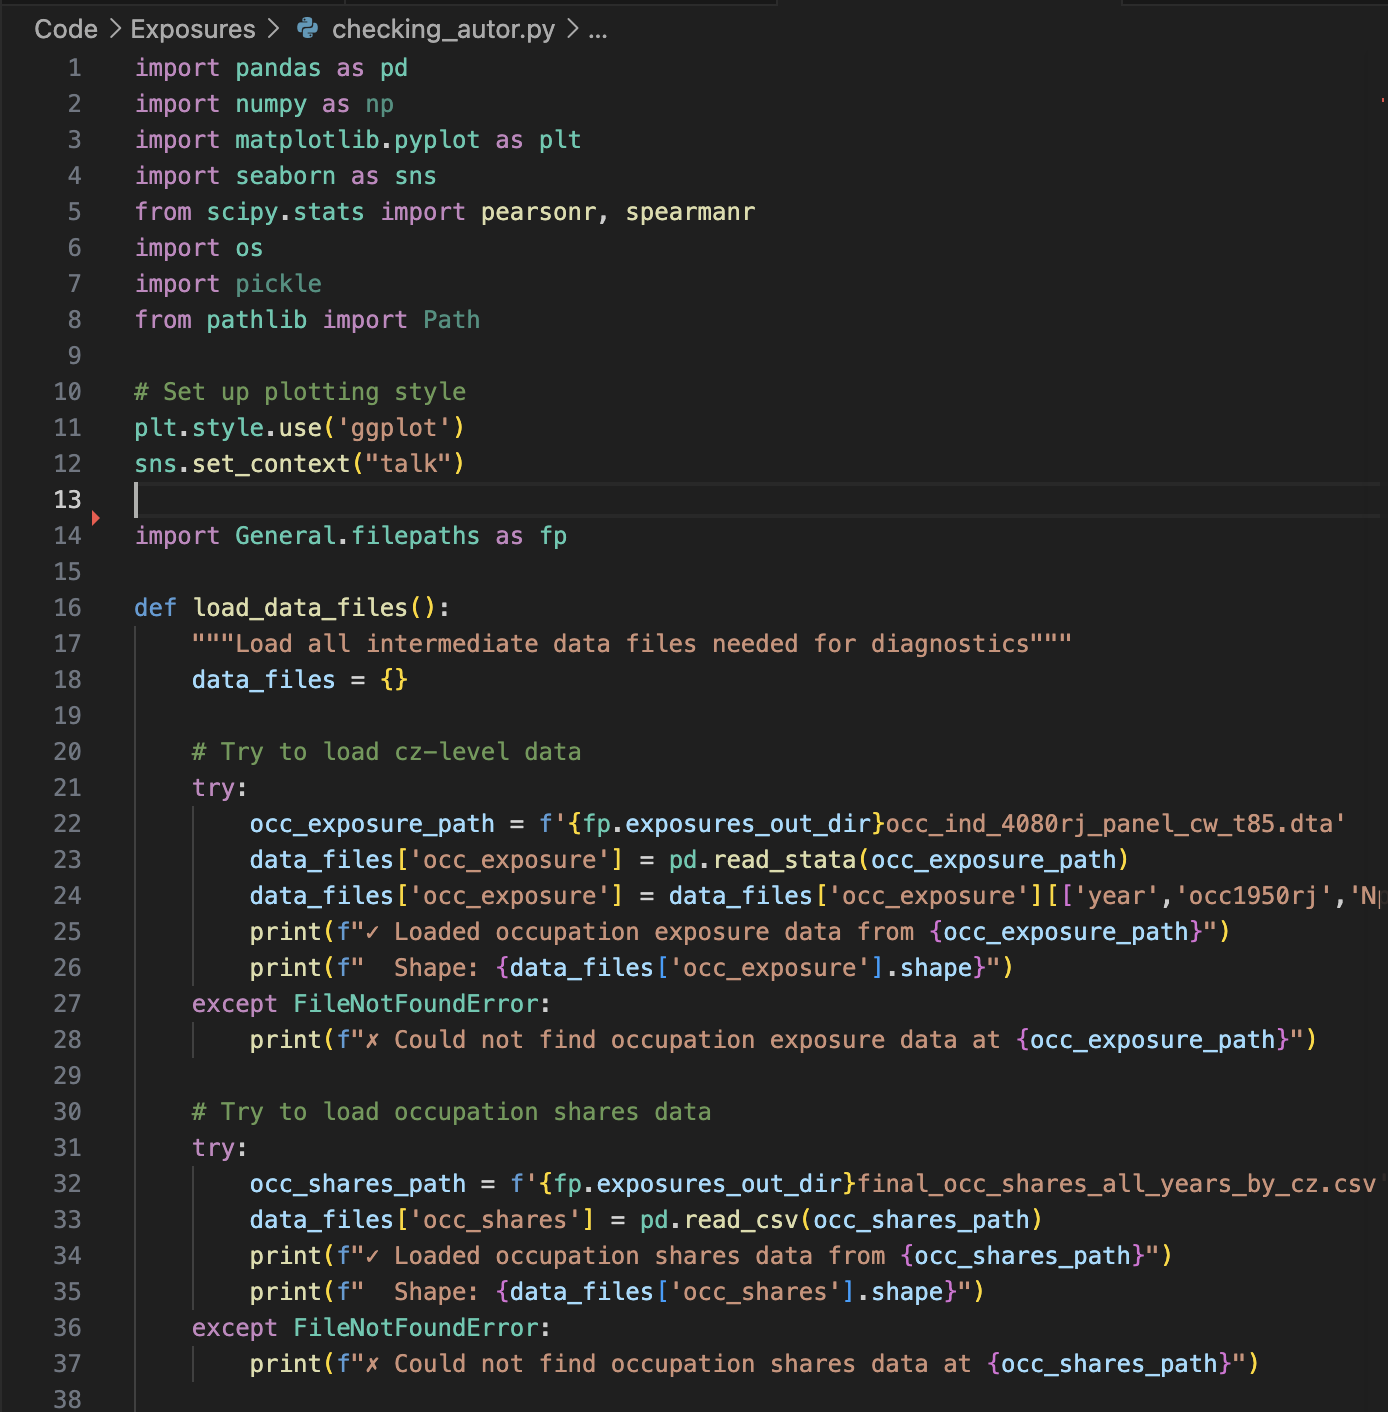
\includegraphics[width=0.75\textwidth]{img/py_script_example.png}
    \end{column}
  \end{columns}
\end{frame}

\begin{frame}{Why Scripts for This Course}
  \small
  \begin{columns}[T]
    \begin{column}{0.48\textwidth}
      \textbf{Notebooks} (\texttt{.ipynb})
      \begin{itemize}
        \item Cells you run one at a time
        \item Great for exploration and teaching
        \item State depends on which cells you ran and in what order
        \item Hard for Claude Code to work with because it cannot ``click'' cells
      \end{itemize}
    \end{column}
    \begin{column}{0.48\textwidth}
      \textbf{Scripts} (\texttt{.py})
      \begin{itemize}
        \item Plain text file, runs top to bottom
        \item Reproducible: \lstinline{python my_script.py} always does the same thing
        \item Claude Code can read, write, and run them directly
        \item \textbf{This is what we use today}
      \end{itemize}
    \end{column}
  \end{columns}

  \vspace{0.8em}
  \begin{alertblock}{The Key Difference}
    Claude Code operates on files, not interactive sessions. Scripts run end-to-end and produce the same result every time, exactly what you need for reproducible research.
  \end{alertblock}
\end{frame}

\begin{frame}{What Changes When You Use Scripts}
  \textbf{You can run scripts line by line} in VS Code (Shift+Enter), just like a notebook. But scripts aren't really built for that.

  \vspace{0.5em}
  Their strength is that they run \textbf{end-to-end}: \lstinline{python my_script.py} always does the same thing, top to bottom. That is what makes them reproducible, and what Claude Code needs.

  \vspace{0.8em}
  \textbf{What this means for your workflow:}
  \begin{itemize}
    \item More \textbf{checkpointing}: save intermediate datasets to disk so you can inspect them
    \item More \textbf{logging}: print row counts, shapes, and summaries as the script runs
    \item More \textbf{intermediate file saves}: write CSVs between pipeline stages
    \item Overall \textbf{less interactive}, more structured
  \end{itemize}

  \vspace{0.5em}
  This feels slower at first. But it produces pipelines that are reproducible, debuggable, and that Claude Code can work with directly.
\end{frame}

% ══════════════════════════════════════════════════════════════════
%  VIRTUAL ENVIRONMENTS
% ══════════════════════════════════════════════════════════════════

\begin{frame}{Virtual Environments}
  \textbf{What is a virtual environment?}\\
  A self-contained folder that holds a separate copy of Python and its packages. Each project gets its own environment, so packages from one project don't interfere with another.

  \vspace{0.5em}
  \textbf{Why you need one:}
  \begin{itemize}
    \item Without it, every project shares the same packages, and updating one project can break another
    \item Claude Code installs packages when it needs them. You want that isolated, not touching your system Python
    \item Reproducibility: you know exactly which packages your project uses
  \end{itemize}

  \vspace{0.5em}
  \textbf{Think of it like this:} a virtual environment is a clean desk for each project. You only put the tools you need on it, and cleaning up one desk does not affect the others.
\end{frame}

\begin{frame}[fragile]{Setting Up a Virtual Environment}
  Run these commands in your terminal, from your project folder:

  \vspace{0.5em}
\begin{lstlisting}
# 1. Create the environment (once per project)
python3 -m venv AIAgents

# 2. Activate it (every time you open a new terminal)
source AIAgents/bin/activate      # Mac/Linux
AIAgents\Scripts\activate         # Windows

# 3. Install packages
pip install pandas numpy statsmodels

# 4. Confirm it's active (you should see (AIAgents) in your prompt)
which python
\end{lstlisting}

  \vspace{0.3em}
  \textbf{In VS Code:} once you create the \texttt{AIAgents} folder, VS Code will detect it and ask to use it as your interpreter. Say yes. After that, every terminal it opens will activate the environment automatically.
\end{frame}

% ══════════════════════════════════════════════════════════════════
%  TERMINAL EXAMPLE: A STATA .do FILE
% ══════════════════════════════════════════════════════════════════

\begin{frame}[fragile]{Detour: Claude Code in the Terminal}
  We'll live in VS Code for this course. But the terminal CLI is always there --- and it's the natural fit for tools \emph{without} an editor integration, like \textbf{Stata}.

  \vspace{0.5em}
  Say you inherited a legacy \texttt{analysis.do} and want to understand and modernize it. Open a terminal in that folder and launch Claude Code:

  \vspace{0.3em}
\begin{lstlisting}
cd ~/my_workspace/session_1/stata_demo
claude
\end{lstlisting}

  \vspace{0.3em}
  No editor, no setup --- just you, the folder, and the agent. Same Claude Code you use in VS Code.
\end{frame}

\begin{frame}[fragile]{Terminal Example: A Stata \texttt{.do} File}
  Once Claude Code is running, ask in plain language:

  \vspace{0.3em}
\begin{lstlisting}[basicstyle=\ttfamily\footnotesize]
> Read analysis.do and explain what each block does.
  Then port it to a documented Python script using
  pandas and statsmodels. Flag anything Stata-specific
  that needs a decision from me before it translates.
\end{lstlisting}

  \vspace{0.4em}
  \textbf{What Claude does:}
  \begin{itemize}
    \item Reads \texttt{analysis.do} and walks you through the regressions
    \item Writes \texttt{analysis.py}, matching the model and output
    \item Flags judgment calls --- e.g.\ \texttt{xtset} panel structure, robust vs.\ clustered SEs --- instead of guessing
  \end{itemize}

  \vspace{0.3em}
  \alert{You still decide. The terminal is just a faster door for a one-off job.}
\end{frame}

% ══════════════════════════════════════════════════════════════════
%  EXERCISE  [37:00–47:00]
% ══════════════════════════════════════════════════════════════════

\begin{frame}[fragile]{Exercise: Your First Commands}
  \textbf{Pick your language.} The starter script builds a county-year vote-share panel --- find it in \texttt{session\_1/scripts/}:

  \vspace{0.2em}
  \begin{itemize}
    \item \textbf{Python:} \texttt{exercise\_build\_panel.py}
    \item \textbf{R:} \texttt{exercise\_build\_panel.R}
    \item \textbf{Stata:} \texttt{exercise\_build\_panel.do}
  \end{itemize}

  \vspace{0.4em}
  \textbf{Task 1:} Ask Claude Code to explain what your script does, line by line.

  \vspace{0.4em}
  \textbf{Task 2:} Ask it to add verification checks, documentation, and print statements.

  \vspace{0.4em}
  \textbf{Task 3:} Ask it to change the two-party vote shares to total vote shares.
\end{frame}

\begin{frame}{Exercise Debrief}
  \begin{itemize}
    \item What did it get right?
    \item Anything wrong or confusing?
    \item That is normal and expected
  \end{itemize}
\end{frame}

% ══════════════════════════════════════════════════════════════════
%  PREVIEW  [47:00–50:00]
% ══════════════════════════════════════════════════════════════════

\begin{frame}{What's Ahead}
  By the end of this course, you will have:
  \begin{itemize}
    \item Built a documented data pipeline
    \item Generated robustness checks
    \item Audited code for errors
    \item Learned version control for agent-assisted work
  \end{itemize}

  \vspace{0.5em}
  You will know which parts Claude Code should handle and which require your judgment.

  \vspace{0.5em}
  \textbf{And you will be able to take these workflows back to your own research.}
\end{frame}

%% ══════════════════════════════════════════════════════════════════
%%  PART B DIVIDER
%% ══════════════════════════════════════════════════════════════════

\begin{frame}{Part B: How Claude Code Works}
  \centering
  \vspace{2em}
  {\Large Now that you have seen what Claude Code can do,\\[0.3em]
  let us look at how it actually works.}

  \vspace{2em}
  Context, modes, and the conventions that make it reliable.
\end{frame}

% ══════════════════════════════════════════════════════════════════
%  FROM INTERACTIVE TO FILE-BASED  [0:00–8:00]
% ══════════════════════════════════════════════════════════════════

\begin{frame}{From Interactive to File-Based Workflows}
  \textbf{What you do now} (Stata / R):
  \begin{itemize}
    \item Open a session, load data into memory
    \item Run commands interactively, see results immediately
  \end{itemize}

  \vspace{0.8em}
  \textbf{How Claude Code works}:
  \begin{itemize}
    \item Reads and writes \textbf{files on disk}
    \item No persistent session with your data loaded
    \item Reads your files $\rightarrow$ writes/modifies scripts $\rightarrow$ optionally runs them
  \end{itemize}
\end{frame}

\begin{frame}{Practical Implication}
  \begin{alertblock}{Think in Projects, Not Sessions}
    You need to think in terms of:
    \begin{itemize}
      \item Project directories
      \item File paths
      \item Scripts that run end-to-end
    \end{itemize}
    Not interactive exploration.
  \end{alertblock}
\end{frame}

% ══════════════════════════════════════════════════════════════════
%  THE CONTEXT WINDOW  [8:00–12:00]
% ══════════════════════════════════════════════════════════════════

\begin{frame}{The Context Window}
  Claude Code can only ``see'' a limited amount of text at once.

  \vspace{0.5em}
  The context window includes:
  \begin{itemize}
    \item Your instructions
    \item The files it reads
    \item Its own responses
  \end{itemize}

  \vspace{0.8em}
  \alert{When a conversation gets long or a project gets large, it loses earlier context.}
\end{frame}

\begin{frame}{Why the Context Window Matters}
  \begin{block}{The Consistency Problem}
    In a complex project with many files, Claude Code may change one file in a way that is \textbf{inconsistent} with another file it can no longer see.
  \end{block}

  \vspace{0.5em}
  Errors compound when the agent loses track of earlier decisions.

  \vspace{0.5em}
  \textbf{We will cover strategies for managing this in Module 3.}
\end{frame}

% ══════════════════════════════════════════════════════════════════
%  PERMISSIONS
% ══════════════════════════════════════════════════════════════════

\begin{frame}{When Claude Code Asks for Permission}
  \begin{columns}[c]
    \begin{column}{0.4\textwidth}
      
\includegraphics[width=\textwidth]{img/claude_permissions.png}
    \end{column}
    \begin{column}{0.56\textwidth}
      Before taking actions (running code, writing files), Claude Code asks you.

      \vspace{0.5em}
      \textbf{Your three options:}
      \begin{enumerate}
        \item \textbf{Yes}: allow this one time
        \item \textbf{Yes, always allow}: allow this type of action for the rest of the session (no more prompts)
        \item \textbf{No}: reject, and tell Claude Code what to do differently
      \end{enumerate}

      \vspace{0.5em}
      \alert{``No'' is not a dead end.}\\
      Use it to redirect: \textit{``No, use a left join instead''} or \textit{``No, don't overwrite that file, create a new one.''}
    \end{column}
  \end{columns}
\end{frame}

\begin{frame}{Common Actions and Risk Levels}
  \scriptsize
  \begin{tabular*}{\textwidth}{@{\extracolsep{\fill}}llll@{}}
    \toprule
    \textbf{Action} & \textbf{Example you'll see} & \textbf{What it does} & \textbf{Risk level} \\
    \midrule
    \texttt{Read}      & \texttt{Read scripts/clean.py}           & Looks at a file          & \color{green!50!black} Safe \\
    \texttt{Glob}      & \texttt{Glob data/**/*.csv}              & Finds files by name      & \color{green!50!black} Safe \\
    \texttt{Grep}      & \texttt{Grep "county\_fips"}             & Searches inside files    & \color{green!50!black} Safe \\
    \texttt{Edit}      & \texttt{Edit clean.py line 42}           & Changes existing code    & \color{yellow!50!black} Review first \\
    \texttt{Write}     & \texttt{Write scripts/merge.py}          & Creates a new file       & \color{yellow!50!black} Review first \\
    \texttt{Bash}      & \texttt{python scripts/clean.py}         & Runs a command           & \color{red!70!black} Read before approving \\
    \texttt{Bash}      & \texttt{pip install pandas}              & Installs a package       & \color{red!70!black} Read before approving \\
    \texttt{Bash}      & \texttt{rm data/old\_panel.csv}          & Deletes a file           & \color{red!70!black} Read before approving \\
    \texttt{Bash}      & \texttt{mv output.csv data/}             & Moves a file             & \color{red!70!black} Read before approving \\
    \texttt{Bash}      & \texttt{git push}                        & Uploads to remote server & \color{red!70!black} Read before approving \\
    \bottomrule
  \end{tabular*}

  \normalsize
  \vspace{0.5em}
  \begin{columns}[T]
    \begin{column}{0.48\textwidth}
      \textbf{\color{green!50!black} Safe to ``always allow'':}\\
      Reading and searching. Claude Code is just looking, not changing anything.
    \end{column}
    \begin{column}{0.48\textwidth}
      \textbf{\color{red!70!black} Always read before approving:}\\
      Bash commands can do \textit{anything}: run code, delete files, install software. Check what it is actually running.
    \end{column}
  \end{columns}
\end{frame}

\begin{frame}[fragile]{Restricting Claude to This Project}
  File access is controlled via \texttt{.claude/settings.json} --- already configured in this course:

  \begin{lstlisting}[basicstyle=\ttfamily\footnotesize]
{
  "permissions": {
    "allow": ["Read(/**)", "Edit(/**)", "Read(~/.claude/**)"]
  }
}
  \end{lstlisting}

  \textbf{What this does:}
  \begin{itemize}
    \item Allows reads and edits \textit{within} the project directory.
    \item Allows Claude to load your user-level config (\texttt{\textasciitilde/.claude/}).
    \item Anything outside the project \textit{prompts for permission} rather than being silently allowed.
  \end{itemize}
\end{frame}

\begin{frame}{Protecting Sensitive Files}
  ``Always allow reads'' assumes there is nothing sensitive to read.\\
  If your project has restricted data or IRB-protected files, you need to keep them away from Claude Code.

  \vspace{0.5em}
  \textbf{For now, the reliable rule is simple:}
  \begin{itemize}
    \item Don't keep restricted or identifiable data inside the folder you run Claude Code in.
    \item Point Claude at a working copy with the sensitive files or columns removed, or keep that data in a separate location entirely.
    \item When in doubt, don't let it read the file --- review before you approve.
  \end{itemize}

  \vspace{0.6em}
  \begin{block}{Coming in Session 4}
    There are dedicated guardrails --- ignore rules and permission denies --- for hiding files from Claude. We'll set them up properly, and see where the naive version quietly fails, once you have a real project.
  \end{block}
\end{frame}

% ══════════════════════════════════════════════════════════════════
%  THE THREE EXECUTION MODES  [12:00–30:00]
% ══════════════════════════════════════════════════════════════════

\begin{frame}{The Three Execution Modes}
  \centering
  {\large The most important configuration decision you will make.}

  \vspace{1em}
  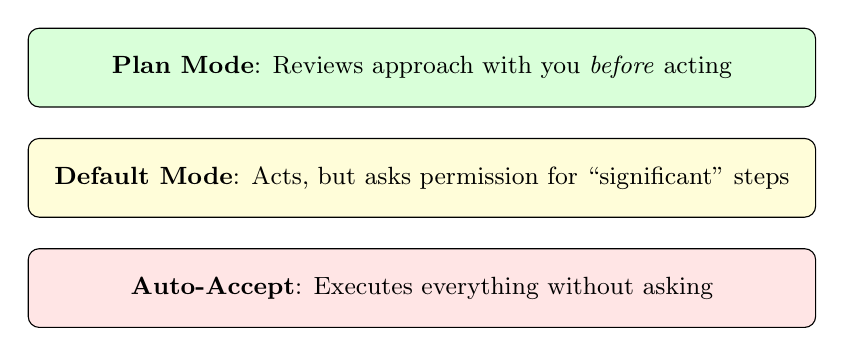
\begin{tikzpicture}[
    node distance=0.4cm,
    every node/.style={draw, rounded corners, minimum width=10cm, minimum height=1cm, align=center, font=\small}
  ]
    \node[fill=green!15] (plan) at (0,2.8) {\textbf{Plan Mode}: Reviews approach with you \textit{before} acting};
    \node[fill=yellow!15] (default) at (0,1.4) {\textbf{Default Mode}: Acts, but asks permission for ``significant'' steps};
    \node[fill=red!10] (auto) at (0,0) {\textbf{Auto-Accept}: Executes everything without asking};
  \end{tikzpicture}

  \vspace{0.5em}
  \small $\downarrow$ More autonomy, less oversight $\downarrow$
\end{frame}

\begin{frame}{Plan Mode \hfill \normalsize\textit{Recommended Default for Research}}
  \textbf{How it works:}
  \begin{itemize}
    \item Claude Code analyzes your request
    \item Proposes a detailed plan (files to read, changes to make, approach)
    \item Waits for your explicit approval before acting
    \item You review, approve, modify, or reject
  \end{itemize}

  \vspace{0.5em}
  \textbf{When to use:}\\
  Any task where the \textit{approach} matters, not just the output.\\
  Data transformation, variable construction, merges, anything analytical.

  \vspace{0.5em}
  \begin{block}{Why It Matters}
    The plan is your checkpoint. This is where you catch ``I am going to do an inner join'' \textit{before} it happens, not after 300 observations are gone.
  \end{block}
\end{frame}

\begin{frame}{Default Mode \hfill \normalsize\textit{Use With Caution}}
  \textbf{How it works:}
  \begin{itemize}
    \item Claude Code executes steps autonomously
    \item Pauses for actions \textit{it} considers significant
    \item Uses its own judgment about when to ask
  \end{itemize}

  \vspace{0.5em}
  \textbf{When to use:}\\
  Routine tasks in established projects where you trust the general approach.

  \vspace{0.8em}
  \begin{alertblock}{The Risk for Academics}
    Claude Code's judgment about what is ``significant'' may not match yours.\\
    It might pause before writing a file but \textbf{not} before silently recoding a variable.
  \end{alertblock}
\end{frame}

\begin{frame}{Auto-Accept Mode \hfill \normalsize\textit{Low-Risk Tasks Only}}
  \textbf{How it works:}
  \begin{itemize}
    \item Executes everything without asking
    \item Reads, writes, runs, and modifies freely
    \item Stops only on errors
  \end{itemize}

  \vspace{0.5em}
  \textbf{When to use:}
  \begin{itemize}
    \item File reformatting
    \item Boilerplate generation
    \item Documentation
  \end{itemize}

  \vspace{0.5em}
  \textbf{When \alert{not} to use:}\\
  Anything involving your data or analysis.\\
  The speed gain is not worth the loss of checkpoints.
\end{frame}

\begin{frame}{The Key Insight on Modes}
  \begin{alertblock}{Different Relationships with the Agent}
    \textbf{Plan mode} = you \textbf{direct} the work\\
    \textbf{Auto-accept} = you \textbf{review} the work after the fact
  \end{alertblock}

  \vspace{0.8em}
  For published research, directing is almost always safer than reviewing after the fact.

  \vspace{0.5em}
  \textbf{Why:} Errors you \textit{prevent} at the planning stage are cheaper than errors you \textit{catch} in the output, or worse, errors you don't catch at all.
\end{frame}

% ══════════════════════════════════════════════════════════════════
%  LIVE DEMO: PLAN vs AUTO-ACCEPT
% ══════════════════════════════════════════════════════════════════

\begin{frame}{Live Demo: Plan Mode vs. Auto-Accept}
  \centering
  \vfill
  Same task, two modes.

  \vspace{0.5em}
  Watch for:
  \begin{itemize}
    \item What does a plan look like?
    \item How do you evaluate it?
    \item What does the experience feel like in each mode?
  \end{itemize}
  \vfill
\end{frame}

% ══════════════════════════════════════════════════════════════════
%  CHOOSING A MODEL
% ══════════════════════════════════════════════════════════════════

\begin{frame}{Choosing a Model}
  Claude Code lets you switch between three model tiers.\\
  Each trades off \textbf{quality}, \textbf{speed}, \textbf{cost}, and \textbf{context window size}.

  \vspace{0.5em}
  \begin{center}
  \small
  \begin{tabular}{@{}llll@{}}
    \toprule
    & \textbf{Haiku 4.5} & \textbf{Sonnet 4.6} & \textbf{Opus 4.6} \\
    \midrule
    Context window & 200k tokens & 200k tokens & 200k--1M tokens \\
    Speed          & Fastest     & Fast        & Slowest \\
    Cost           & Lowest      & Moderate    & Highest \\
    Reasoning      & Basic       & Strong      & Strongest \\
    \bottomrule
  \end{tabular}
  \end{center}

  \vspace{0.3em}
  \textbf{To switch models in Claude Code:}\\
  Type \texttt{/model} and select, or press \texttt{Shift+Tab} to toggle.
\end{frame}

\begin{frame}{When to Use Each Model}
  \begin{columns}[T]
    \begin{column}{0.32\textwidth}
      \textbf{Haiku}\\[0.3em]
      {\small Fast, cheap, good enough for simple tasks.}
      \begin{itemize}
        \item Reformatting files
        \item Renaming variables
        \item Generating boilerplate
        \item Quick questions about syntax
      \end{itemize}
    \end{column}
    \begin{column}{0.32\textwidth}
      \textbf{Sonnet}\\[0.3em]
      {\small The everyday workhorse for most research tasks.}
      \begin{itemize}
        \item Writing data cleaning scripts
        \item Building panels and merges
        \item Debugging code
        \item Drafting documentation
      \end{itemize}
    \end{column}
    \begin{column}{0.32\textwidth}
      \textbf{Opus}\\[0.3em]
      {\small Maximum reasoning power; use when it matters.}
      \begin{itemize}
        \item Complex multi-file refactors
        \item Subtle specification decisions
        \item Reviewing analytical code
        \item Large-context projects (up to 1M tokens)
      \end{itemize}
    \end{column}
  \end{columns}
\end{frame}

\begin{frame}{Model Choice: The Research Perspective}
  \begin{columns}[c]
    \begin{column}{0.38\textwidth}
      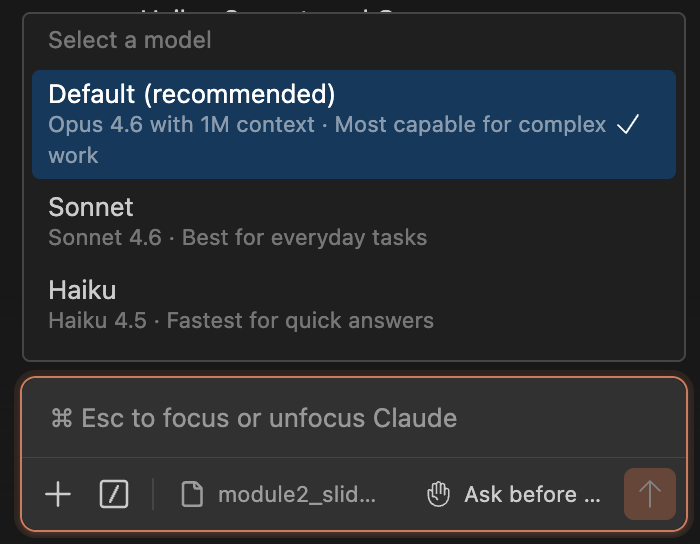
\includegraphics[width=\textwidth]{img/claude_models.png}
    \end{column}
    \begin{column}{0.58\textwidth}
      \begin{alertblock}{The Key Tradeoff}
        Smarter models are slower and more expensive.\\
        A wrong answer fast is worse than a right answer slow.
      \end{alertblock}

      \vspace{0.3em}
      \textbf{Rules of thumb:}
      \begin{itemize}
        \item \textbf{Default to Sonnet}: best balance of quality and speed
        \item \textbf{Upgrade to Opus} for careful reasoning or many files
        \item \textbf{Drop to Haiku} for mechanical, easy-to-verify tasks
      \end{itemize}
    \end{column}
  \end{columns}
\end{frame}

% ══════════════════════════════════════════════════════════════════
%  THINKING AND EFFORT
% ══════════════════════════════════════════════════════════════════

\begin{frame}{Thinking vs.\ Not Thinking}
  Beyond \emph{which} model, you control \emph{how hard} it works before it answers.

  \vspace{0.6em}
  \begin{columns}[T]
    \begin{column}{0.48\textwidth}
      \textbf{Not thinking (default)}\\[0.3em]
      {\small The model responds directly. Fast and cheap.}
      \begin{itemize}
        \item Reformatting, renaming
        \item Simple, well-specified edits
        \item Quick factual questions
      \end{itemize}
    \end{column}
    \begin{column}{0.48\textwidth}
      \textbf{Thinking (extended reasoning)}\\[0.3em]
      {\small The model reasons step-by-step \textit{before} acting. Slower, more tokens, fewer mistakes.}
      \begin{itemize}
        \item Debugging stubborn errors
        \item Specification decisions
        \item Planning a multi-step change
      \end{itemize}
    \end{column}
  \end{columns}

  \vspace{0.6em}
  \begin{alertblock}{When in doubt}
    If the task involves a \textbf{judgment call} or Claude got it wrong once already, turn thinking on. For mechanical work, leave it off.
  \end{alertblock}
\end{frame}

\begin{frame}{Dialing the Effort}
  \textbf{Trigger thinking with plain words.} Adding a thinking cue to your prompt tells Claude how much reasoning budget to spend --- more words, more thinking:

  \vspace{0.4em}
  \begin{center}
  \small
  \begin{tabular}{@{}ll@{}}
    \toprule
    \textbf{What you type} & \textbf{Effect} \\
    \midrule
    (nothing)        & Answers directly \\
    ``\texttt{think}''        & A little reasoning first \\
    ``\texttt{think hard}''   & More careful reasoning \\
    ``\texttt{ultrathink}''   & Maximum reasoning budget \\
    \bottomrule
  \end{tabular}
  \end{center}

  \vspace{0.5em}
  \textbf{The effort setting.} Both \textbf{Sonnet} and \textbf{Opus} have an \textbf{effort} setting you can pick with \texttt{/model}, from least to most thorough:
  \begin{center}
    \small\texttt{low} \,$\to$\, \texttt{medium} \,$\to$\, \texttt{high} \,$\to$\, \texttt{extra high} \,$\to$\, \texttt{max} \,$\to$\, \texttt{ultracode}
  \end{center}
  Higher effort = more thorough, slower, costlier. Think of it as the same knob, set once for the session rather than per-prompt.

  \vspace{0.4em}
  \alert{Thinking is not free.} It spends tokens and time --- reach for it when correctness matters, not by reflex.
\end{frame}

% ══════════════════════════════════════════════════════════════════
%  GETTING FILES IN
% ══════════════════════════════════════════════════════════════════

\begin{frame}{Getting Files In: Drag and Drop}
  You don't have to describe a file in words --- you can hand it straight to Claude.

  \vspace{0.6em}
  \textbf{Hold \texttt{Shift} and drop into the chat panel} (in VS Code) to add something as context:
  \begin{itemize}
    \item A \textbf{data file} (\texttt{.csv}, \texttt{.xlsx}) so Claude can see the columns
    \item A \textbf{figure or PDF} --- a paper, a table, a chart to reproduce
    \item A \textbf{screenshot} of an error message or a plot that looks wrong
  \end{itemize}

  \vspace{0.5em}
  \begin{alertblock}{Two ways to do it}
    \begin{itemize}
      \item \textbf{Shift+drag} a file from the VS Code Explorer (or your Finder/desktop) onto the chat box --- holding \texttt{Shift} is what drops it in as context instead of opening it
      \item \textbf{Paste} an image directly with \texttt{Cmd+V} / \texttt{Ctrl+V} --- great for screenshots
    \end{itemize}
  \end{alertblock}

  \vspace{0.3em}
  {\small A screenshot of a broken plot plus ``why does this look wrong?'' is often faster than describing it.}
\end{frame}

% ══════════════════════════════════════════════════════════════════
%  COST MANAGEMENT
% ══════════════════════════════════════════════════════════════════

\begin{frame}{Cost Management}
  \begin{alertblock}{A Real Constraint}
    On the \$20/month plan, you can burn through your allocation in 30--45 minutes of active use if you are not strategic.
  \end{alertblock}

  \vspace{0.5em}
  \textbf{Principles:}
  \begin{enumerate}
    \item Not everything needs Claude Code. Small edits are faster by hand
    \item A well-written CLAUDE.md reduces back-and-forth (= fewer tokens)
    \item If Claude Code is spinning on a wrong approach, \textbf{intervene early}
    \item Batch related tasks into one well-scoped request
    \item Plan mode adds tokens but prevents costly wrong approaches
  \end{enumerate}
\end{frame}

\begin{frame}{Usage Limits and Model Cost}
  \begin{columns}[c]
    \begin{column}{0.45\textwidth}
      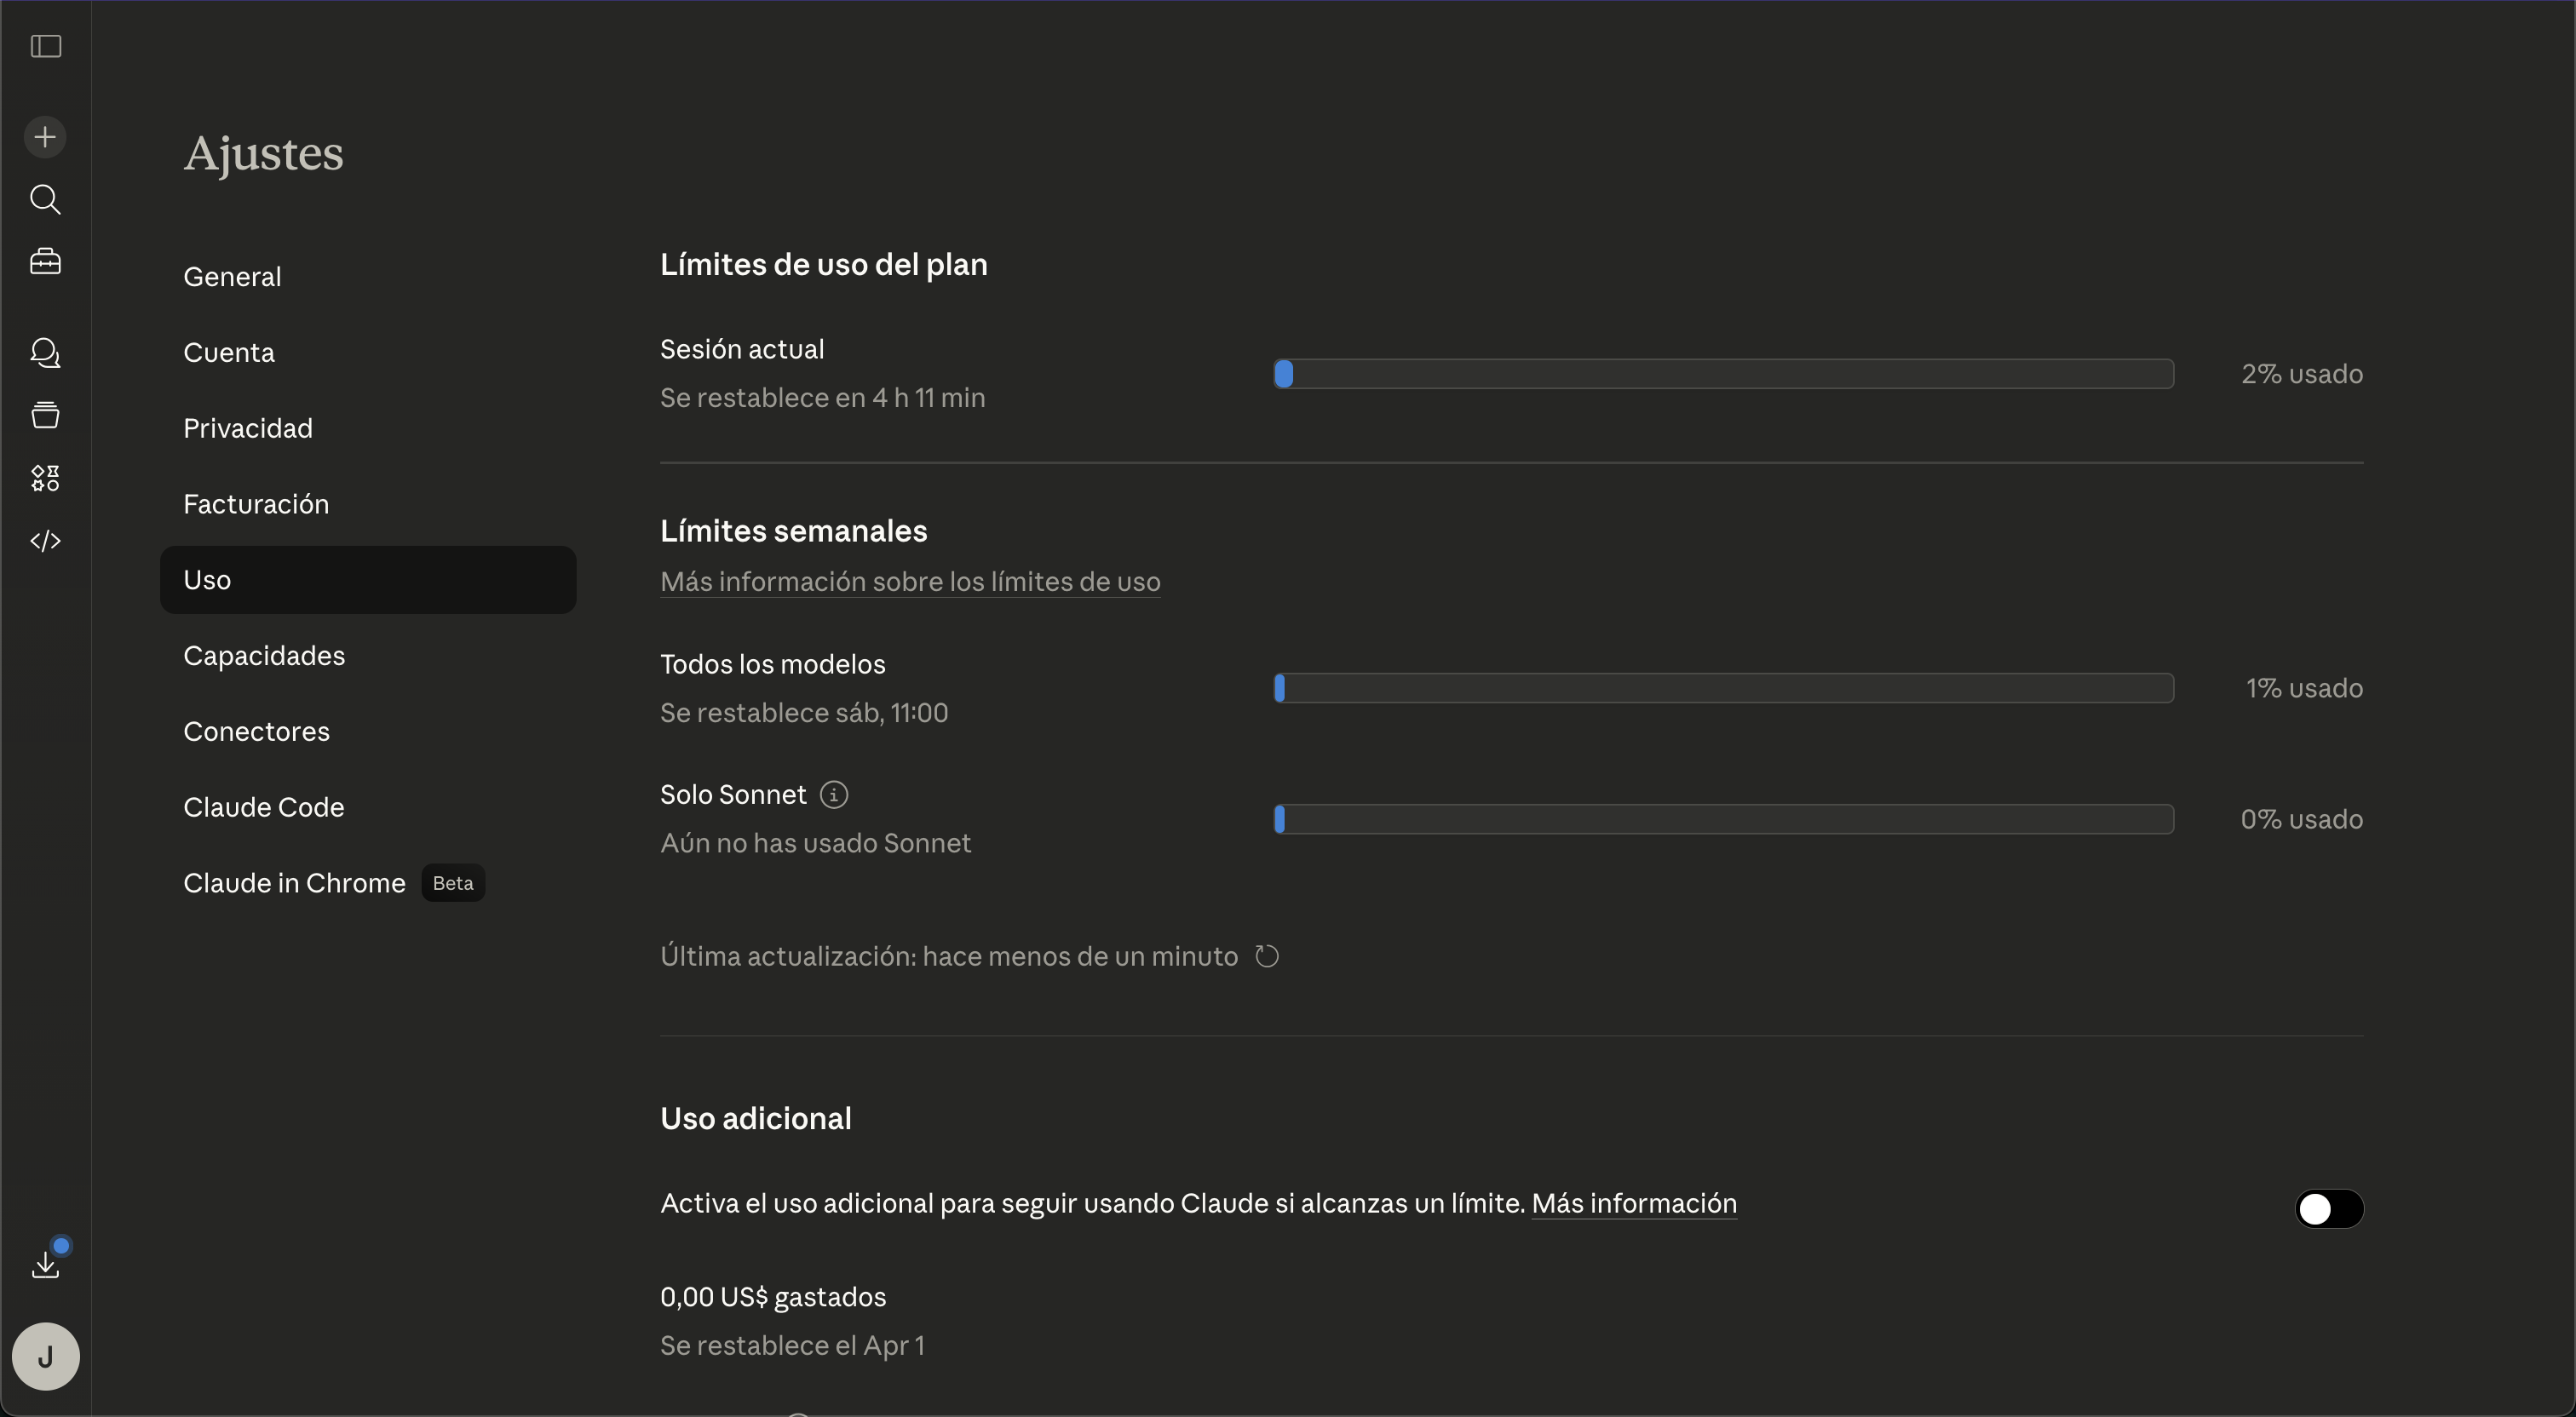
\includegraphics[width=\textwidth]{img/usage_limits.png}
    \end{column}
    \begin{column}{0.52\textwidth}
      \textbf{How limits work:}
      \begin{itemize}
        \item Token allowance resets on a \textbf{5-hour rolling window}
        \item A separate \textbf{weekly cap} limits total usage
        \item When you hit either limit, Claude Code pauses until the window resets
      \end{itemize}

      \vspace{0.5em}
      \textbf{Which models burn tokens fastest:}
      \begin{itemize}
        \item \textbf{Opus} uses $\sim$5$\times$ more tokens per task than Haiku
        \item \textbf{Sonnet} is the middle ground
        \item \textbf{Haiku} stretches your budget the furthest
      \end{itemize}

      \vspace{0.5em}
      \alert{Match the model to the task.}\\
      Don't use Opus to rename variables.
    \end{column}
  \end{columns}
\end{frame}

% ══════════════════════════════════════════════════════════════════
%  CLAUDE.MD  [30:00–40:00]
% ══════════════════════════════════════════════════════════════════

\begin{frame}{Where Claude Looks for Context}
  Claude Code reads instructions from \textbf{several levels} when it starts a session. Anything it finds is loaded into the context window before your first message.

  \vspace{0.6em}
  \begin{itemize}
    \item \textbf{User level} --- \texttt{\textasciitilde/.claude/CLAUDE.md}\\
      {\small Applies to \textit{every} project on your machine. Personal preferences, defaults, things you want Claude to know about you regardless of what you are working on.}
    \item \textbf{Project level} --- \texttt{CLAUDE.md} in the project root\\
      {\small Checked into git, shared with collaborators. Project conventions, data structure, constraints.}
    \item \textbf{Subfolder level} --- \texttt{CLAUDE.md} inside a subdirectory\\
      {\small Loaded when Claude works in that subtree. Useful for scoped rules (e.g.\ a \texttt{cleaning/} folder with its own conventions).}
  \end{itemize}

\end{frame}

\begin{frame}{How Claude Reads the Hierarchy}
  When Claude Code starts, it walks from the user level down to your working directory and loads \textbf{every applicable CLAUDE.md} it finds. They are concatenated into context, with more specific (deeper) files appearing later --- so they take precedence when guidance conflicts.

  \vspace{0.8em}
  \begin{alertblock}{This hierarchy is everywhere}
    The same user $\rightarrow$ project $\rightarrow$ subfolder pattern shows up across the power-user sessions:
    \begin{itemize}
      \item \textbf{Skills} --- defined at the user or project level, loaded on demand
      \item \textbf{Hooks} --- configured per user or per project
      \item \textbf{MCP servers \& permissions} --- scoped per user or per project
      \item \textbf{Subagents} --- registered at the user or project level
    \end{itemize}
  \end{alertblock}

  \vspace{0.4em}
  \textbf{Learn the hierarchy once} and it tells you where every other piece of configuration belongs.
\end{frame}

\begin{frame}{CLAUDE.md: Your Lab Notebook for the Agent}
  \begin{columns}[c]
    \begin{column}{0.45\textwidth}
      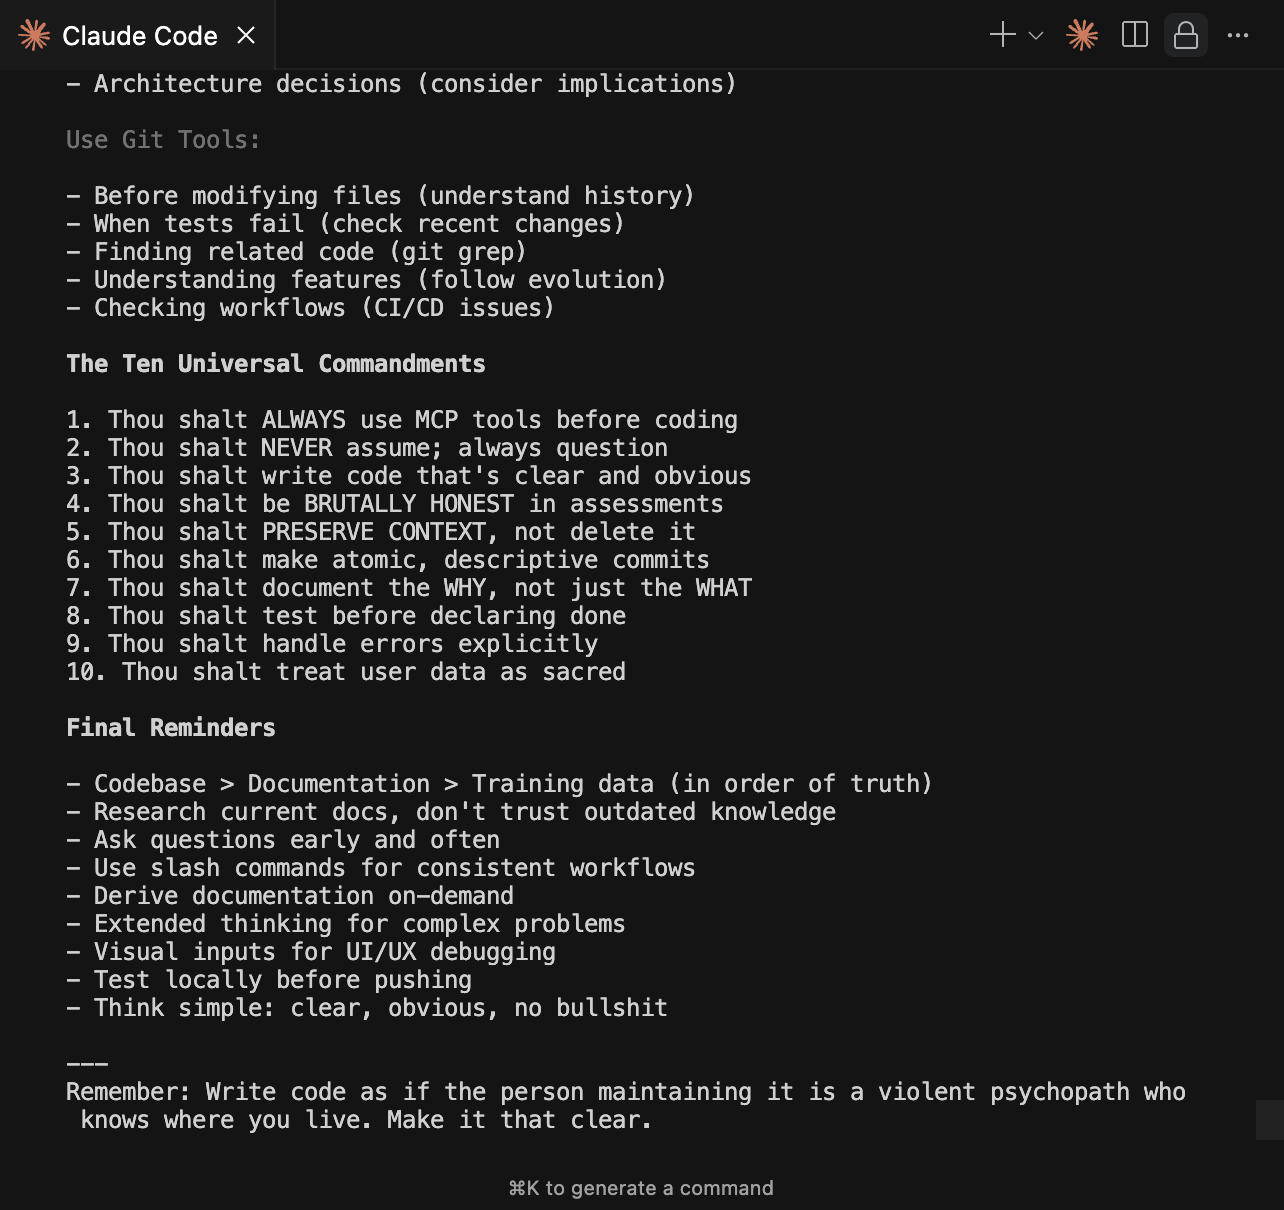
\includegraphics[width=\textwidth]{img/claude_md.png}\\
      {\tiny Credit: u/rishabhsonker}
    \end{column}
    \begin{column}{0.52\textwidth}
      Plain text files at the \textbf{user}, \textbf{project}, or \textbf{subfolder} level that Claude Code reads \textbf{automatically at the start of every conversation}.

      \vspace{0.5em}
      They encode your conventions, definitions, and constraints so you do not have to repeat them each time.

      \vspace{0.5em}
      \textbf{The single most effective way to prevent errors before they happen.}

      \vspace{0.5em}
      {\small \textit{Note:} This does not guarantee Claude Code will always follow these instructions, but it significantly increases the chances.}
    \end{column}
  \end{columns}
\end{frame}

\begin{frame}{What Belongs in CLAUDE.md}
  \textbf{In the \textit{project-level} CLAUDE.md, include:}
  \begin{columns}[T]
    \begin{column}{0.48\textwidth}
      \begin{itemize}
        \item Project description \& research question
        \item Data structure: files, key variables, units, expected ranges
        \item Coding conventions
      \end{itemize}
    \end{column}
    \begin{column}{0.48\textwidth}
      \begin{itemize}
        \item Constraints: ``never drop observations without logging''
        \item ``All merges must report row counts''
        \item What Claude Code should \textbf{not} do
      \end{itemize}
    \end{column}
  \end{columns}

  \vspace{0.4em}
  {\footnotesize Keep \textit{user-level} CLAUDE.md for things that apply across projects; use a \textit{subfolder} CLAUDE.md only when a directory needs its own rules.}

  \vspace{0.4em}
  \begin{block}{How it interacts with the context window}
    Every applicable CLAUDE.md is loaded before your first message and stays ``visible''---but it takes up space, so keep each one focused and concise.
  \end{block}
\end{frame}

\begin{frame}[fragile]{CLAUDE.md Example}
\begin{lstlisting}
# CLAUDE.md - County Migration Project

## Research Question
Effect of historical migration on county-level outcomes.

## Data
- data/raw/census_panel.csv: county-year panel, 1920-2020
- Key vars: fips (5-digit), year, population, migration_share
- All monetary values in 2020 USD

## Constraints
- Never drop observations without logging count and reason
- All merges must report pre- and post-merge row counts
- Always use robust standard errors
- Do not choose model specifications
- Do not interpret coefficients
\end{lstlisting}
\end{frame}

% ══════════════════════════════════════════════════════════════════
%  EXERCISE  [48:00–70:00]
% ══════════════════════════════════════════════════════════════════

\begin{frame}{Exercise: Build the County Panel From Scratch}
  In Module 1 you ran a pre-built script. Now \textbf{you} build it.

  \vspace{0.3em}
  \textbf{Same data, fresh start.} Work in pairs using plan mode.

  \vspace{0.5em}
  \begin{enumerate}
    \item Write a \texttt{CLAUDE.md} for the project (use the template)
    \item Switch Claude Code to \textbf{plan mode}
    \item Ask Claude Code to build a county-year panel that merges election returns with IPUMS census demographics
    \item \textbf{Before approving the plan}, you will need to:
      \begin{itemize}
        \item Read the codebooks to understand variable codings\\
          {\small (What does \texttt{EDUC $\geq$ 10} mean? What does \texttt{RACE == 1} code?)}
        \item Decide how to define key variables\\
          {\small (Two-party vote share? College = bachelor's or higher?)}
        \item Specify the merge: which keys, which join type, expected row counts
      \end{itemize}
    \item Review the plan, reject or revise as needed, then approve
    \item Run the script and verify the output
  \end{enumerate}
\end{frame}

\begin{frame}{Evaluating the Plan}
  When Claude Code proposes its plan, ask yourself:

  \vspace{0.5em}
  \begin{itemize}
    \item Is it reading the \textbf{codebooks} or just guessing at variable meanings?
    \item How is it coding \texttt{EDUC}, \texttt{RACE}, \texttt{HISPAN}?\\
      {\small Do those match \textit{your} definitions?}
    \item What join type is it using? Inner, left, or outer?\\
      {\small What happens to counties that appear in one dataset but not the other?}
    \item Is it filtering \texttt{mode == "TOTAL"} for election data?
    \item Does it handle \texttt{COUNTYFIP == 0} (unidentified counties)?
  \end{itemize}

  \vspace{0.5em}
  \alert{This is where your domain knowledge matters.}\\
  Claude Code can write the code, but you decide what the variables mean.
\end{frame}

% ══════════════════════════════════════════════════════════════════
%  DEBRIEF  [70:00–75:00]
% ══════════════════════════════════════════════════════════════════

\begin{frame}{Debrief}
  \begin{itemize}
    \item What variable coding decisions did you make? Did Claude Code's default match yours?
    \item Did anyone reject or modify the plan? What did you change?
    \item How did your panel compare to the Module 1 version?
  \end{itemize}

  \vspace{0.8em}
  \begin{block}{The Lesson}
    \textbf{Writing a CLAUDE.md} forces you to be explicit about conventions you have kept implicit.

    \vspace{0.3em}
    \textbf{Reviewing plans} forces you to think about approach \textit{before} you see output.

    \vspace{0.3em}
    \textbf{Domain knowledge} is key for preventing errors.
  \end{block}
\end{frame}

% ══════════════════════════════════════════════════════════════════
%  SUMMARY
% ══════════════════════════════════════════════════════════════════

\begin{frame}{Module 2 Summary}
  \begin{enumerate}
    \item Claude Code works with \textbf{files}, not interactive sessions
    \item The \textbf{context window} limits what it can hold, so keep tasks focused
    \item \textbf{Plan mode} is the default for research work
    \item \textbf{CLAUDE.md} is your most powerful tool for preventing errors
    \item \textbf{Cost management} is a core skill, not an afterthought
  \end{enumerate}

  \vspace{1em}
  \centering
  \textbf{Next: Module 3, Automating Research Tasks}
\end{frame}

\end{document}
